\chapter{Sviluppo dell'hardware dell'incubatrice neonatale}
\section{Architettura del sistema}
In questo capitolo vengono descritte le caratteristiche fisiche del prototipo di incubatrice neonatale. Si parte dalla descrizione
della struttura fisica, si prosegue con la descrizione dei componenti elettronici presenti ed infine si analizzano le connessioni
tra i vari componenti e il microcontrollore. Per una migliore organizzazione, l'insieme delle componenti elettriche
ed elettroniche è stato suddiviso in tre macrocategorie, affrontate nei successivi paragrafi:
\begin{enumerate}
	\item attuatori e relè;
	\item pannello frontale e sensore di temperatura e umidità SHT20;
	\item scheda Arduino Mega 2560 con microcontrollore ATmega2560.
\end{enumerate}


\subsection{Descrizione della struttura fisica}
L'incubatrice neonatale è composta da una camera interna principale ed un cassetto inferiore contenente i componenti elettronici
e la vasca con l'acqua per l'umidificazione.

La camera interna è costituita con pareti laterali in polistirene espanso sinterizzato (ESP) sostenute ai quattro angoli da un
telaio in legno. La base della camera interna è costituita da un pannello in legno ed è stato usato un pannello in policarbonato
trasparente come rivestimento superiore. Il pannello superiore è incernierato alla struttura in legno lungo il lato lungo e
permette il rapido accesso alla camera interna. Sul lato frontale sono presenti due sportelli che permettono un accesso rapido
alla camera interna senza provocare grandi dispersioni di calore e umidità.

Il cassetto inferiore è realizzato con una struttura in legno estraibile dove sono posizionati i vari componenti elettronici
e la vasca con l'acqua per l'umidificazione.

\begin{figure}[htbp]
	\centering
	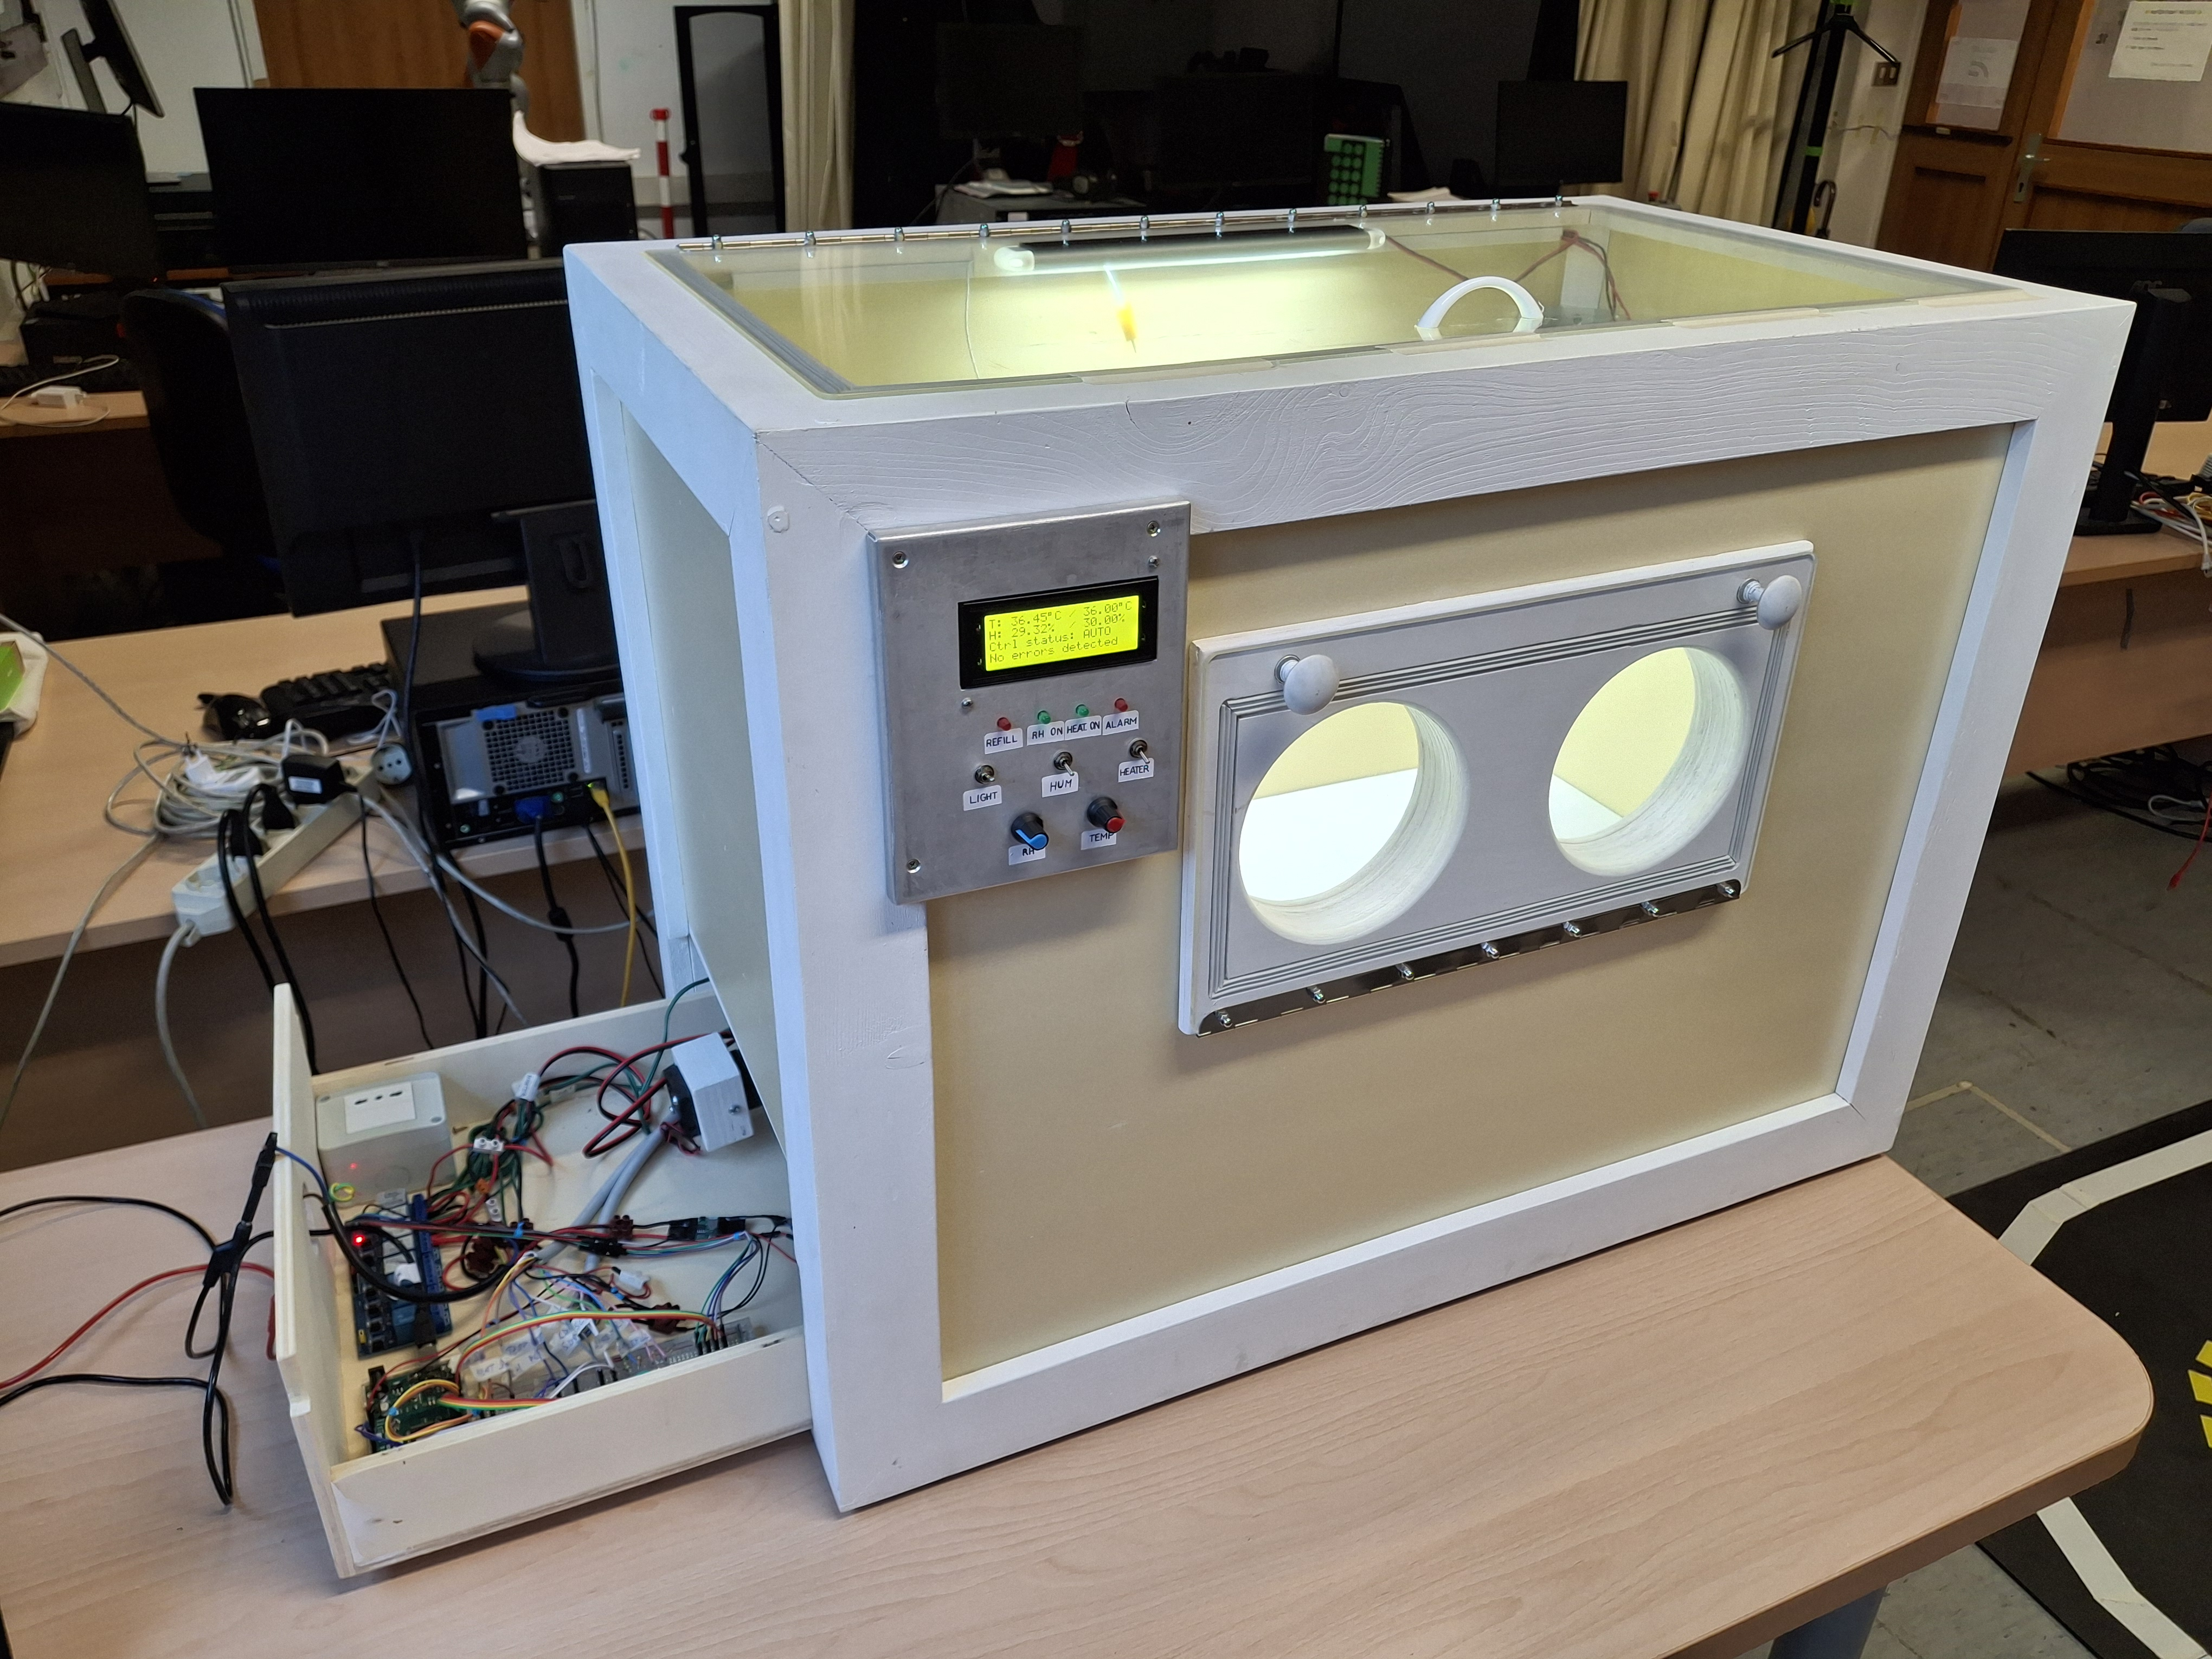
\includegraphics[width=0.9\textwidth, trim={0cm 7cm 0cm 8cm}, clip]{immagini/1_incubatrice.jpg}
	\caption[Foto del prototipo di incubatrice neonatale]{Foto del prototipo di incubatrice neonatale dove si può apprezzare
	la camera interna illuminata, il cassetto inferiore con i componenti elettronici, i due oblò per l'accesso rapido, il
	pannello in policarbonato superiore e il pannello frontale.}
	\label{fig:interno_incubatrice}
\end{figure}

\subsection{Attuatori e relè}
Di seguito sono analizzati i vari attuatori presenti nel prototipo di incubatrice neonatale che permettono di agire sul sistema
per modificarne le condizioni ambientali interne.

\subsubsection{Riscaldatore con ventola associata}
Per riscaldare l'aria della camera interna, è utilizzato un riscaldatore a resistenza elettrica da 100W. Esso è situato
su un angolo della camera interna e sorretto da un supporto in alluminio attaccato al telaio in legno. Dietro al riscaldatore è
presente una ventola che permette di spingere l'aria attraverso le resistenze elettriche del riscaldatore.

\subsubsection{Umidificatore con ventola associata}
Per l'umidificazione dell'aria della camera interna, si utilizza un umidificatore a ultrasuoni per generare vapore acqueo. Si trova
nel cassetto inferiore all'interno di un contenitore in plastica ermetico che funge da serbatoio dell'acqua. Il vapore acqueo
prodotto viene spinto dalla ventola all'interno di un tubo in plastica che collega il contenitore con la camera interna.

\subsubsection{Ventola di omogeneizzazione dell'aria}
Per favorire il ricircolo dell'aria nella camera interna, ed evitare la formazione di stratificazioni di temperatura e umidità,
è presente una ventola di omogeneizzazione dell'aria. Si trova sull'angolo adiacente al riscaldatore ed è anch'essa sorretta da
un supporto in alluminio.

\subsubsection{Barra led}
Per l'illuminazione della camera interna, è presente una barra led posta sul pannello trasparente superiore della camera interna.

\subsubsection{Relè e step down per il controllo degli attuatori}
I vari attuatori con le relative ventole sopra elencati richiedono tutti una tensione di alimentazione di 12 V. L'unico che fa
eccezione è l'umidificatore che lavora a 24 V. Date le elevate correnti richieste, per garantire un funzionamento stabile e sicuro
i vari gli attuatori a 12 V sono collegati ad un alimentatore da banco esterno opportunamente dimensionato, mentre l'umidificatore
è alimentato dal suo alimentatore esterno da 24V.

Per poter essere gestiti dal microcontrollore, tra l'alimentatore e i vari attuatori, sono stati inseriti dei relè controllati
con segnali a 5 V dalla scheda Arduino Mega. Siccome le bobine dei relè richiedono una corrente maggiore di quella che può essere
erogata dal microcontrollore, è stato aggiunto un convertitore step down da 12 V a 5 V per alimentare le bobine dei relè a 5 V
utilizzando l'energia erogata dall'alimentatore esterno a 12 V.

\begin{figure}[htbp]
    \centering
    \begin{subfigure}[b]{0.48\textwidth}
        \centering
        %
\includegraphics[width=\textwidth]{1_riscaldatore.jpg}
        \caption{Riscaldatore a resistenza elettrica con ventola posta dietro di esso.}
        \label{fig:riscaldatore}
    \end{subfigure}
    \hfill % Spinge le immagini verso i margini, creando spazio al centro
    \begin{subfigure}[b]{0.48\textwidth}
        \centering
        %\includegraphics[width=\textwidth]{2_umidificatore.jpg}
        \caption{Umidificatore a ultrasuoni con ventola per spingere il vapore acqueo verso la camera interna.}
        \label{fig:umidificatore}
    \end{subfigure}
    \vspace{0.5cm}
	\begin{subfigure}[b]{0.48\textwidth}
        \centering
        %
\includegraphics[width=\textwidth]{1_ventola_omogeneizzazione.jpg}
        \caption{Ventola di omogeneizzazione dell'aria per favorire il ricircolo dell'aria nella camera interna.}
        \label{fig:ventola_omogeneizzazione}
    \end{subfigure}
    \hfill
    \begin{subfigure}[b]{0.48\textwidth}
        \centering
        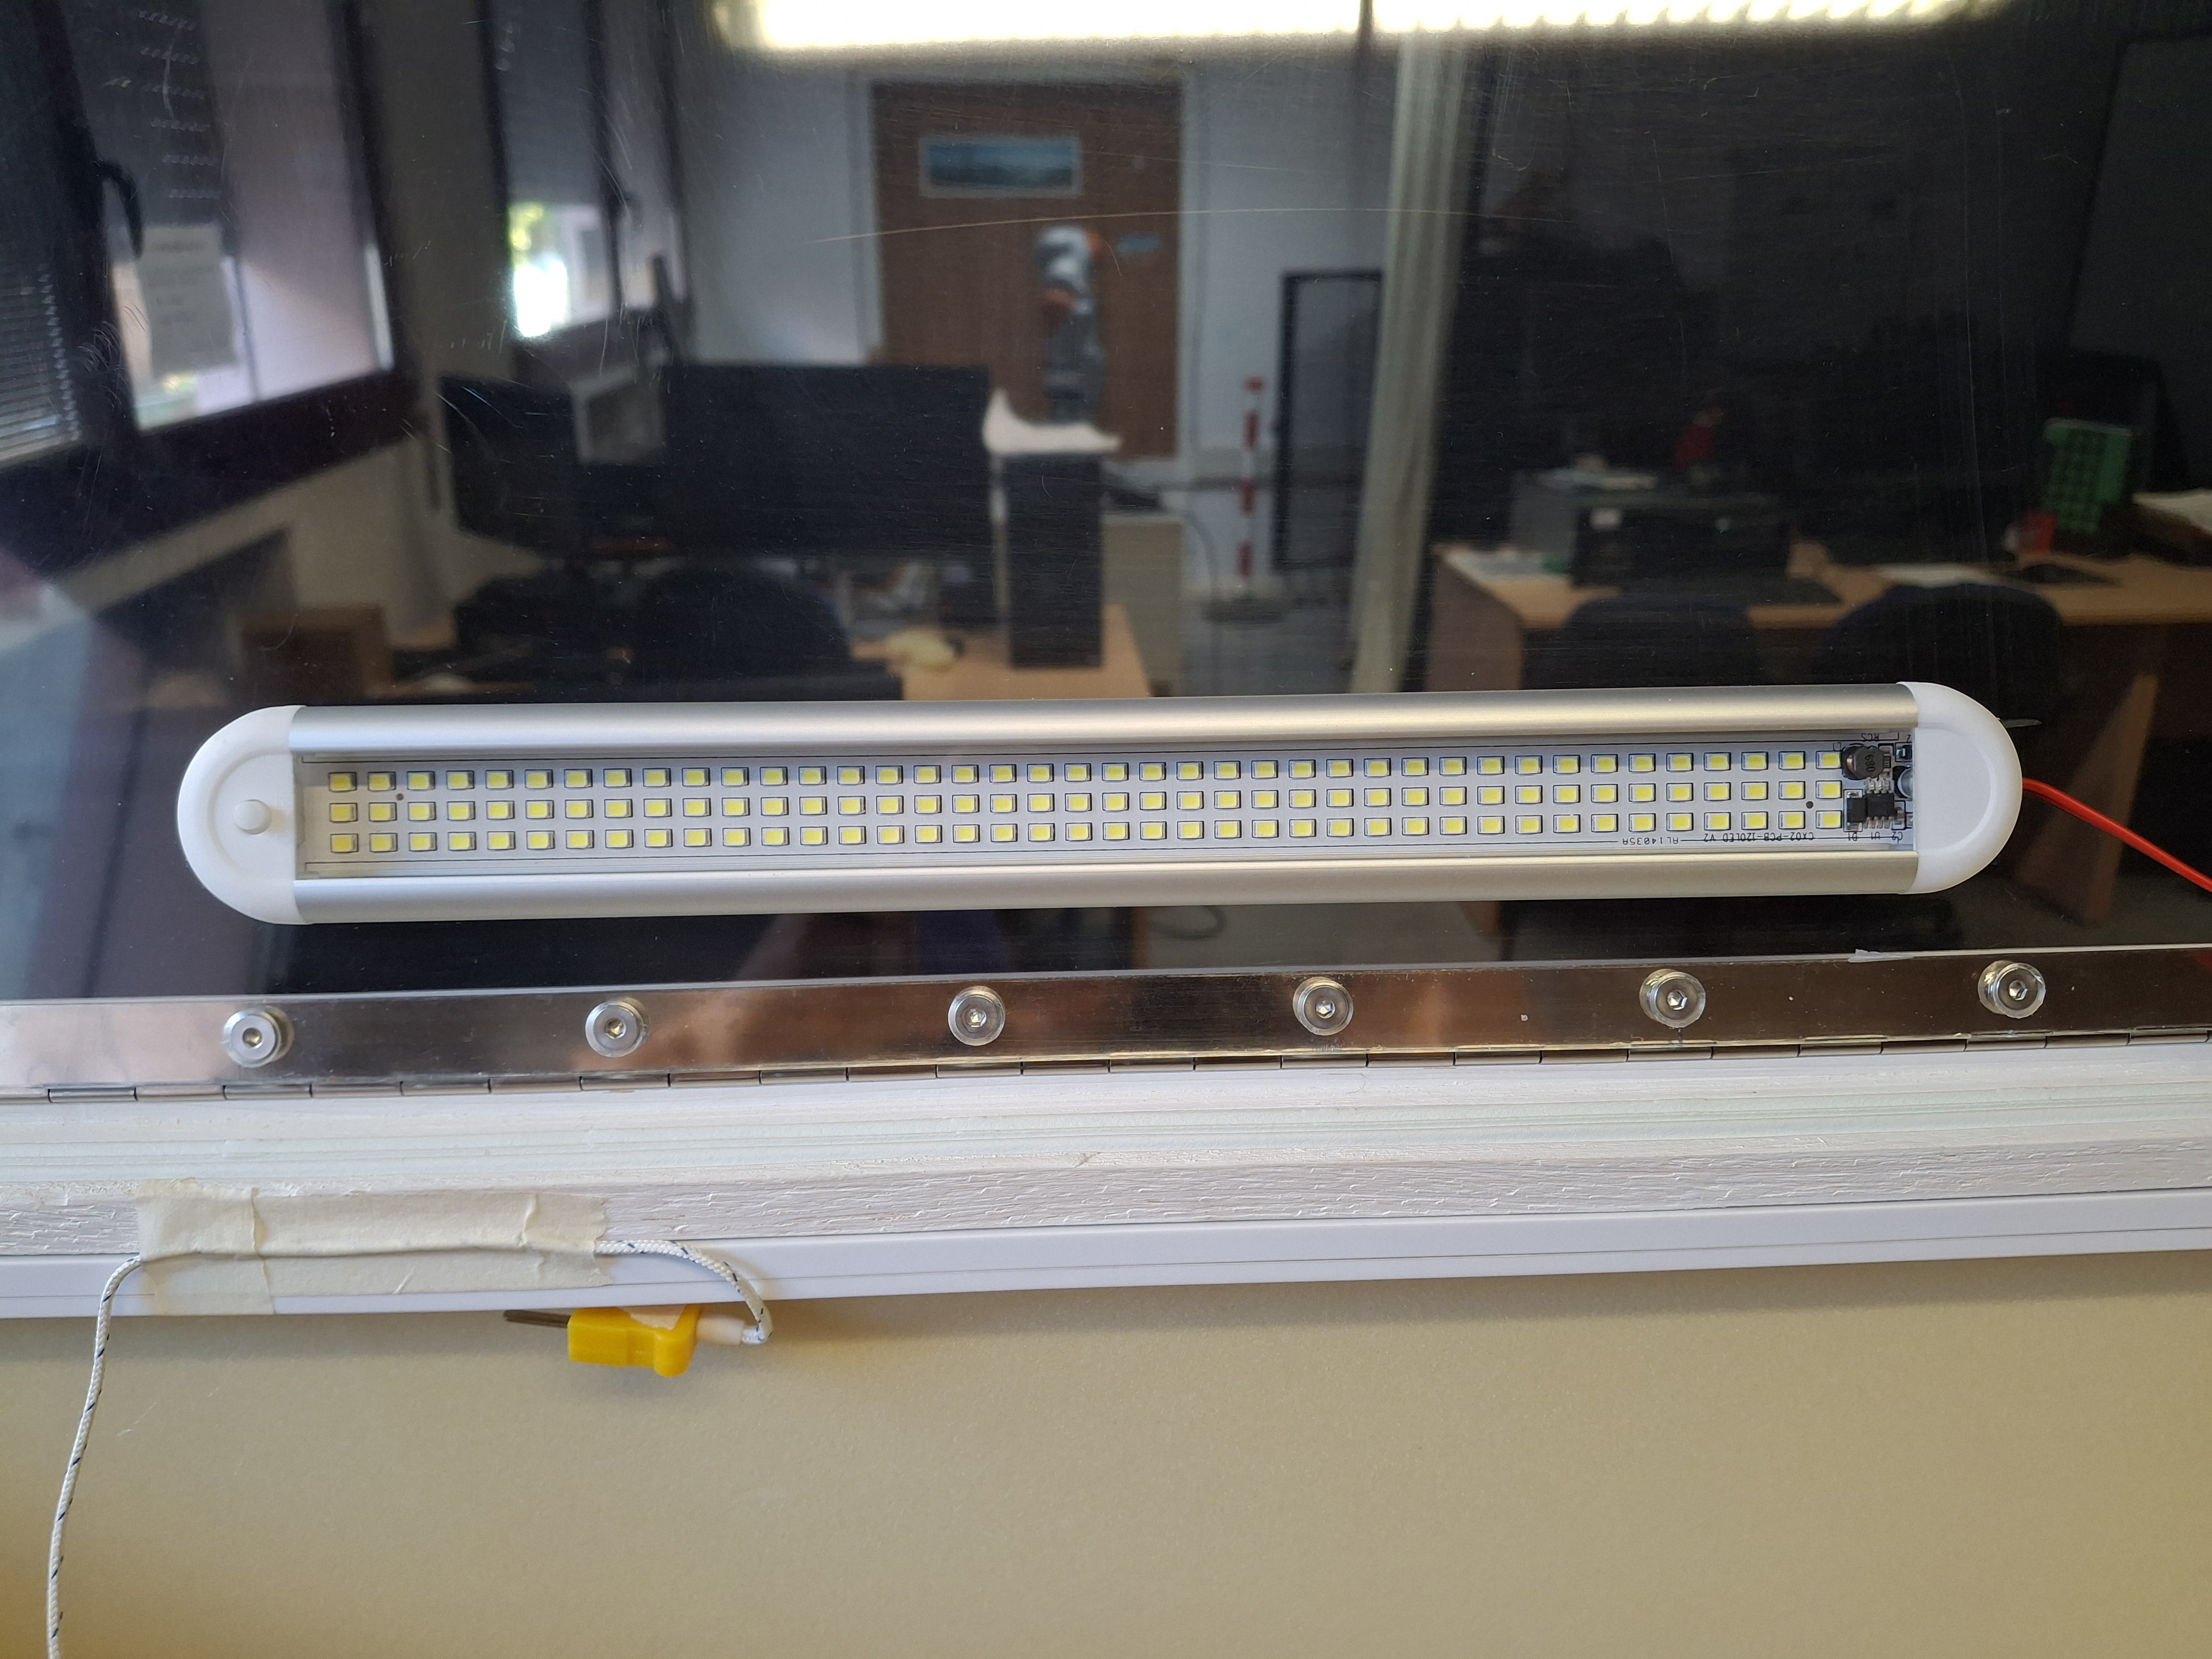
\includegraphics[width=0.9\textwidth, trim={0cm 25cm 0cm 25cm}, clip]{immagini/1_barra_led.jpg}
        \caption{Barra LED per l'illuminazione della camera interna.}
        \label{fig:barra_led}
    \end{subfigure}

    \caption[Foto degli attuatori]{Foto degli attuatori presenti nel prototipo di incubatrice neonatale.}
    \label{fig:griglia_completa}
\end{figure}

\begin{figure}[htbp]
	\centering
	\begin{subfigure}[b]{0.65\textwidth}
        \centering
		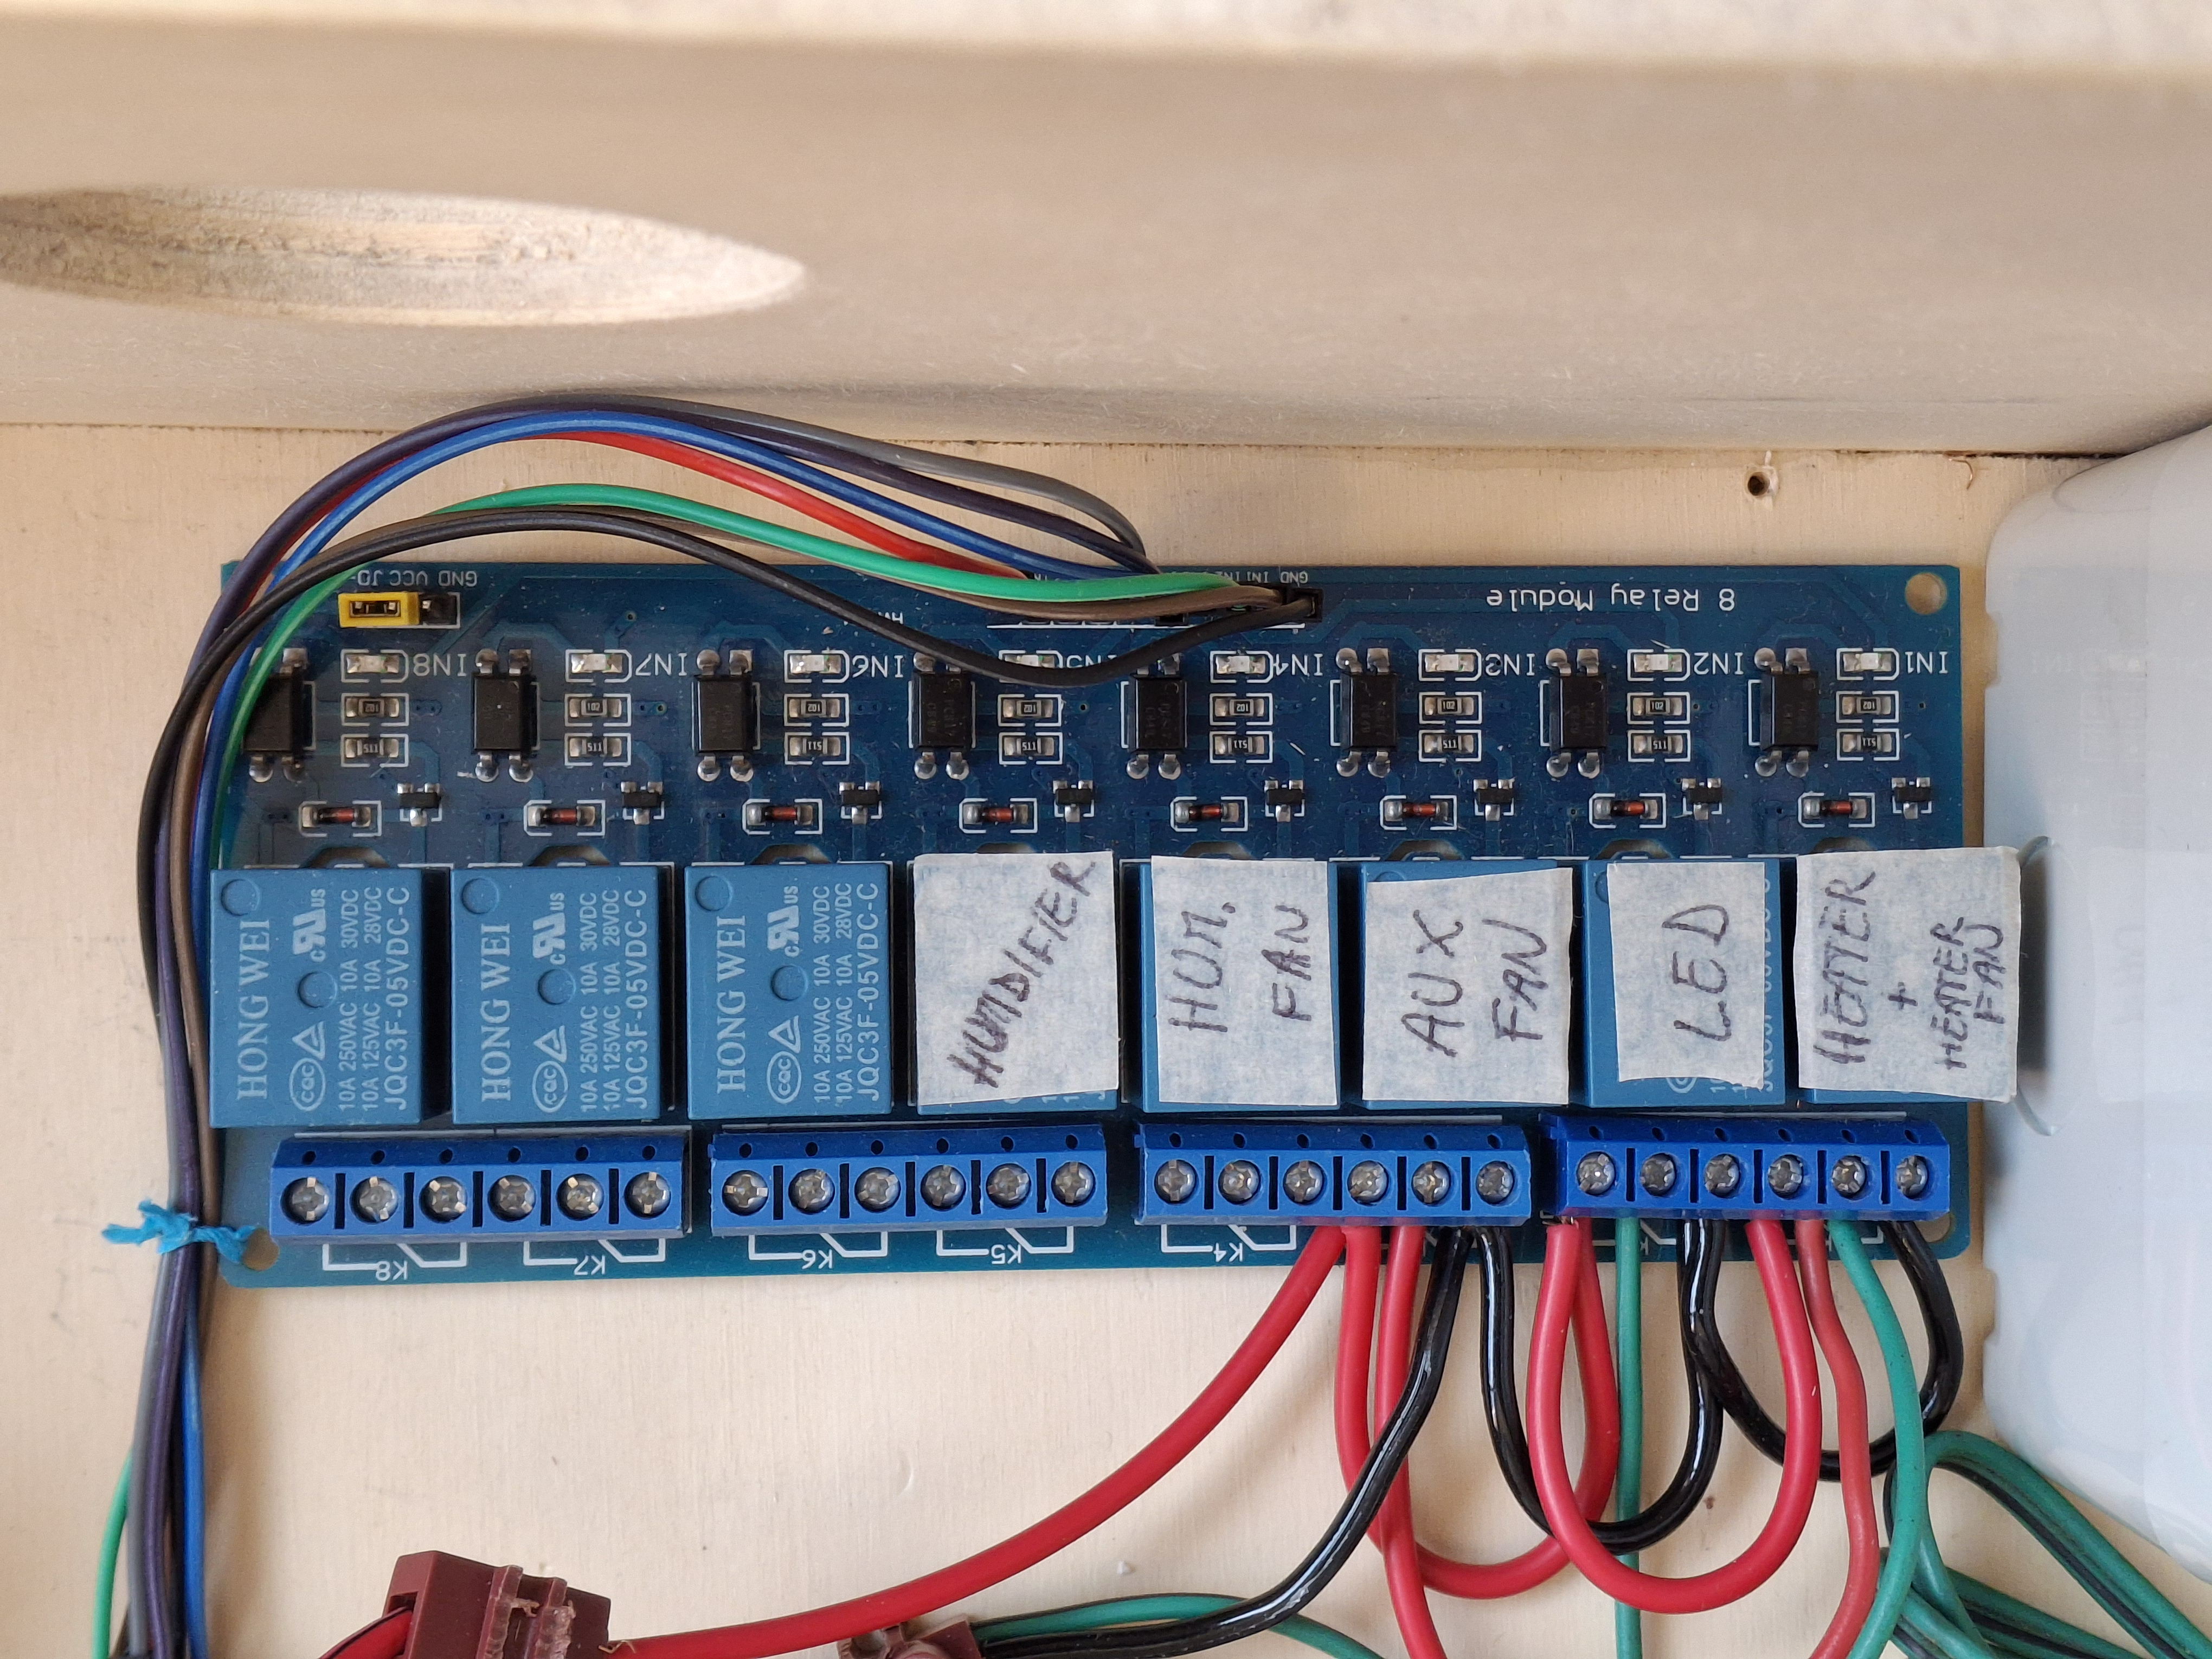
\includegraphics[width=0.9\textwidth, trim={1cm 2cm 2cm 20cm}, clip]{immagini/1_rele.jpg}
        \caption{Foto dei relè per il controllo degli attuatori del prototipo di incubatrice neonatale.}
        \label{fig:rele}
    \end{subfigure}
    \hfill % Spinge le immagini verso i margini, creando spazio al centro
    \begin{subfigure}[b]{0.34\textwidth}
        \centering
        %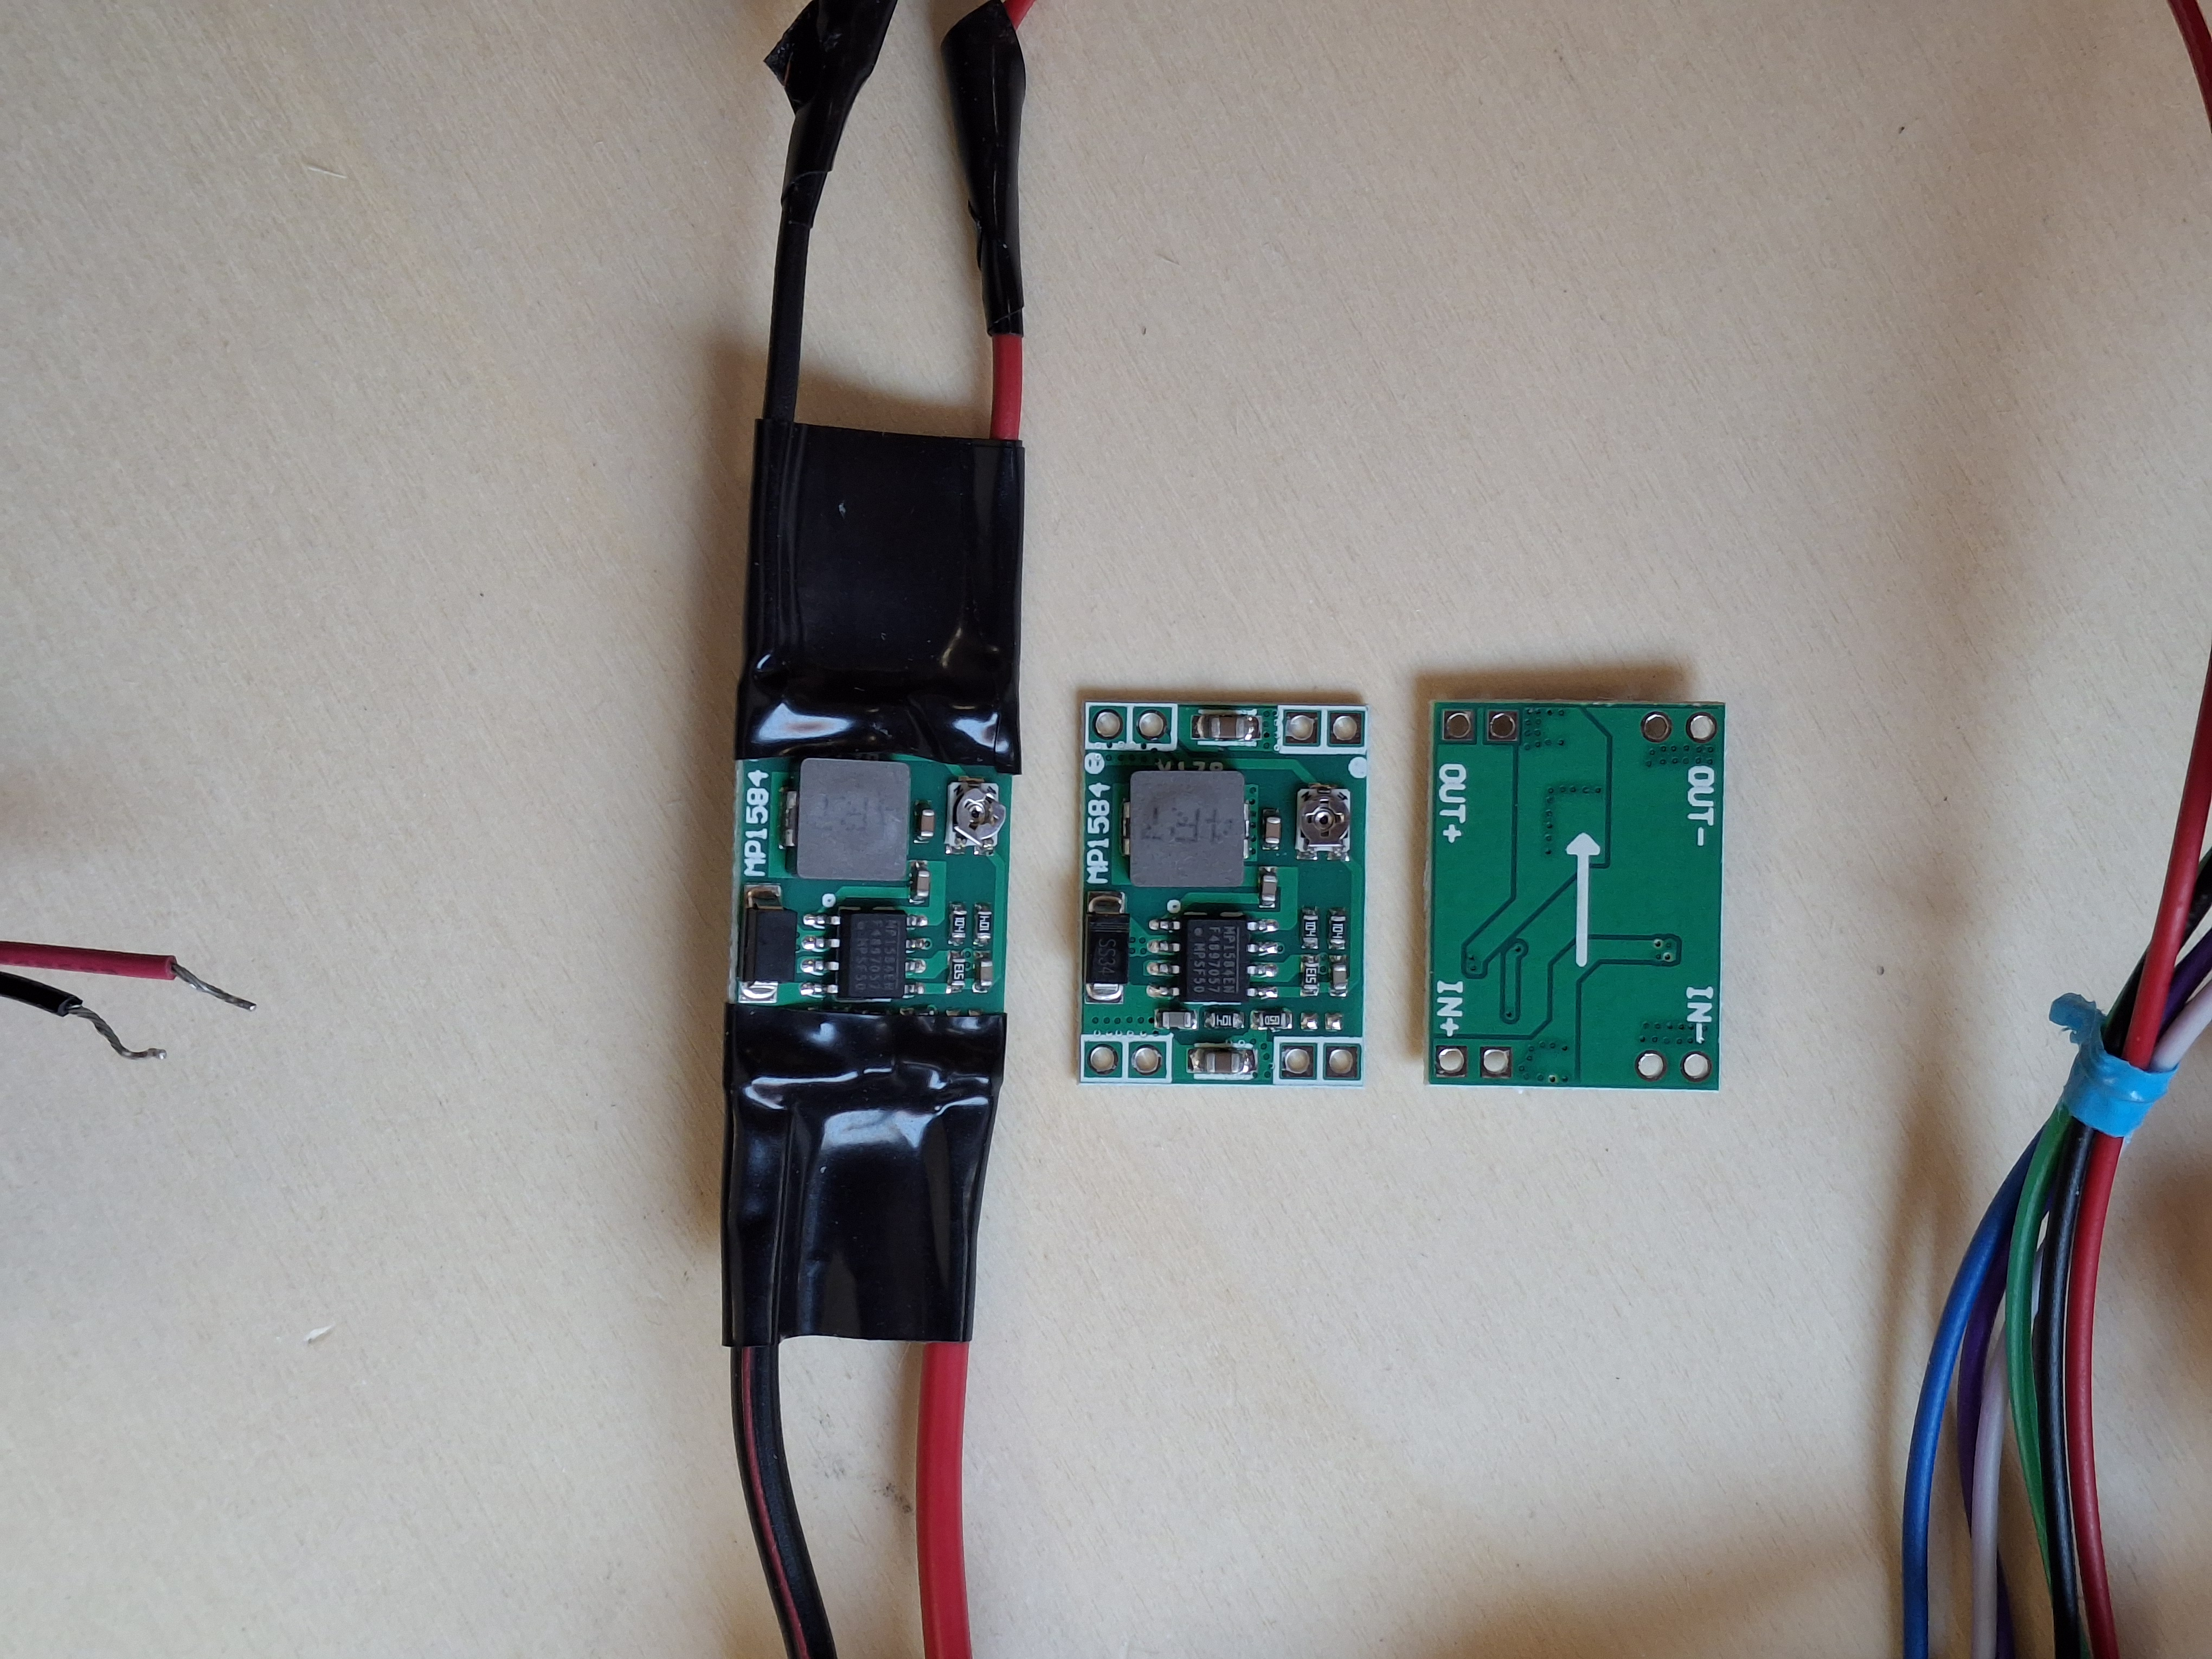
\includegraphics[width=\textwidth]{immagini/1_step_down.jpg}
        \caption{Foto dello step down per alimentare le bobine dei relè a 5 V.}
        \label{fig:step_down}
    \end{subfigure}
	\caption[Foto dei relè e dello step down]{Foto dei relè e dello step down per il controllo degi attuatori
	del prototipo di incubatrice neonatale.}
	\label{fig:rele_step_down}
\end{figure}


\subsection{Pannello frontale e sensore SHT20}
Il pannello frontale del prototipo di incubatrice neonatale fornisce l'interfaccia utente con cui l'utilizzatore può interagire
con il sistema. Si trova nella parte frontale del dispositivo ed è facilmente accessibile. Esso è composto dai seguenti
componenti:
\begin{itemize}
	\item un display LCD 20x4 con interfaccia I2C;
	\item 4 led di stato per indicare l'accensione del riscaldatore, l'accensione dell'umidificatore, la presenza di un allarme
	e la necessità di eseguire un refill del serbatoio dell'acqua dell'umidificatore;
	\item 3 switch a due posizioni per il controllo manuale del riscaldatore, dell'umidificatore e della barra led presente
	all'interno del prototipo di incubatrice neonatale;
	\item 2 potenziometri rotativi per la regolazione del setpoint di temperatura ed umidità.
\end{itemize}

\begin{figure}[htbp]
	\centering
	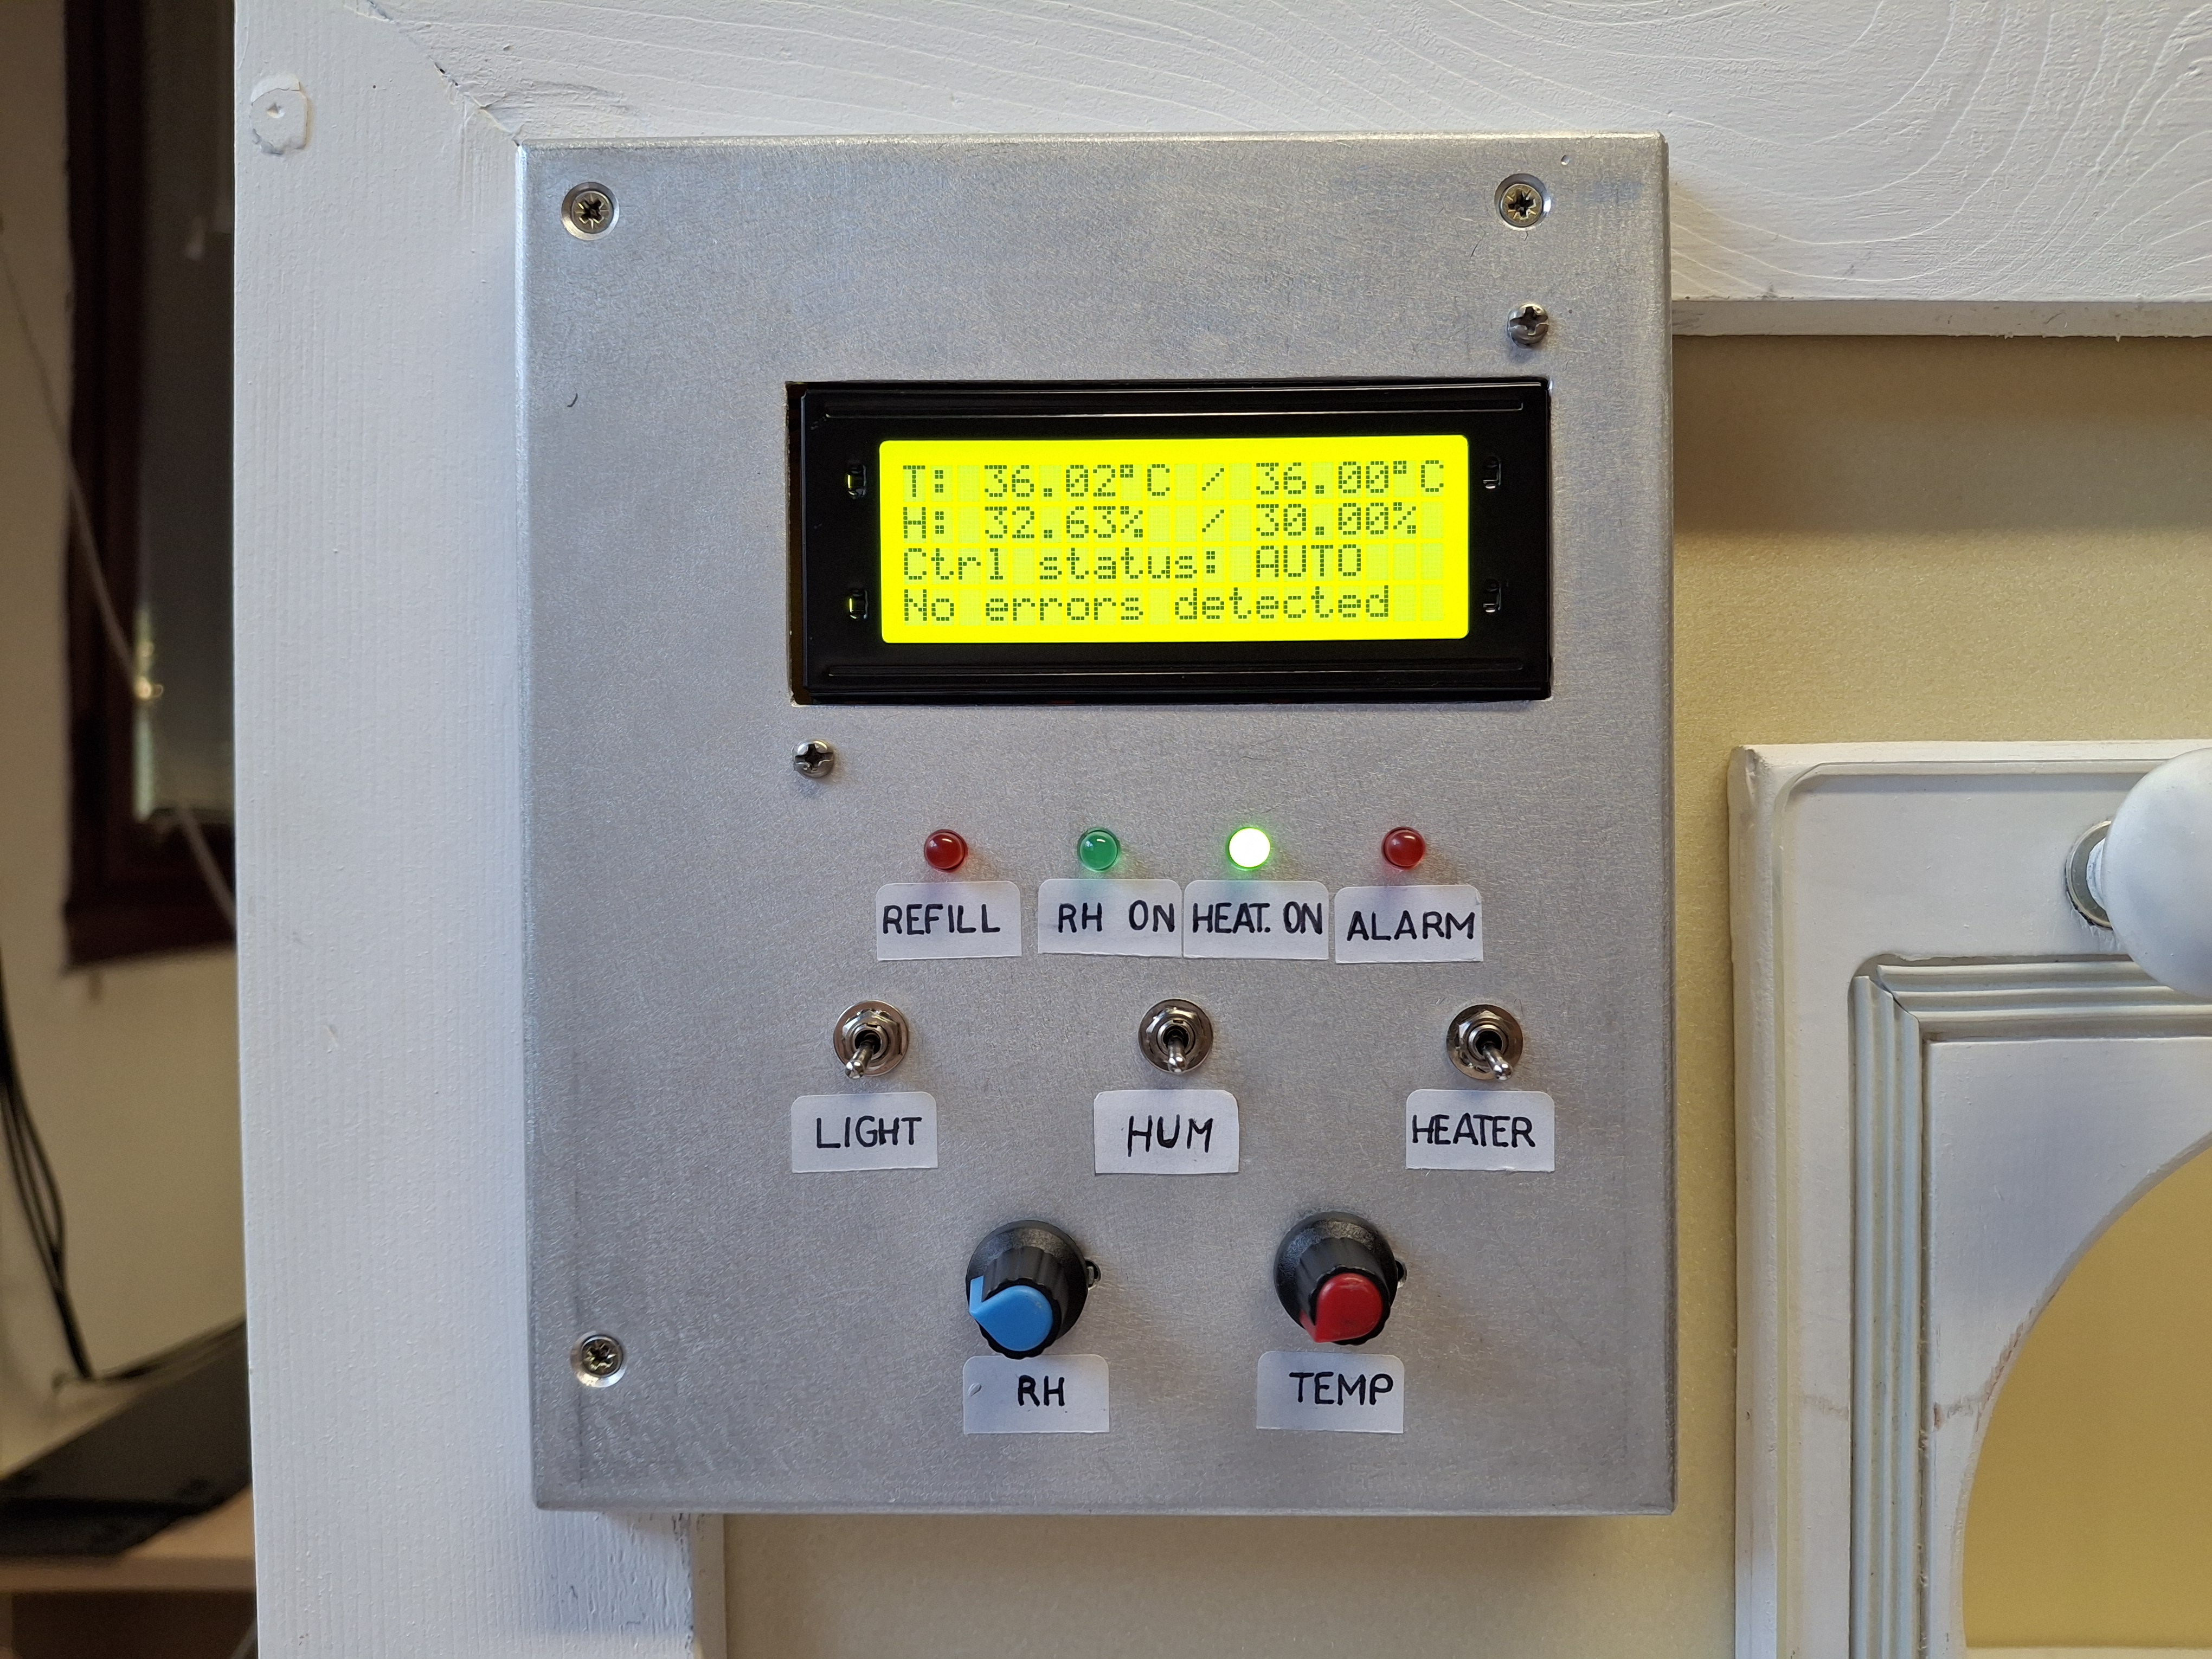
\includegraphics[width=0.9\textwidth, trim={0cm 7cm 0cm 6cm}, clip]{immagini/1_pannello_frontale_1.jpg}
	\caption[Foto del pannello frontale]{Foto del pannello frontale del prototipo di incubatrice neonatale con i vari componenti
	presenti.}
	\label{fig:pannello_frontale}
\end{figure}

Il sensore di temperatura e umidità SHT20 è un sensore digitale che permette di misurare la temperatura e l'umidità relativa
dell'ambiente in cui si trova. Esso è posizionato all'interno della camera interna del prototipo di incubatrice neonatale.
Per i test effettuati, il sensore è stato posizionato a 20 cm dalle pareti laterali lunghe, a 17 cm dalla parete corta opposta
al riscaldatore e alla ventola di omogeneizzazione dell'aria e a 7.5 cm di altezza dal piano della base della camera interna.

\begin{figure}[htbp]
	\centering
	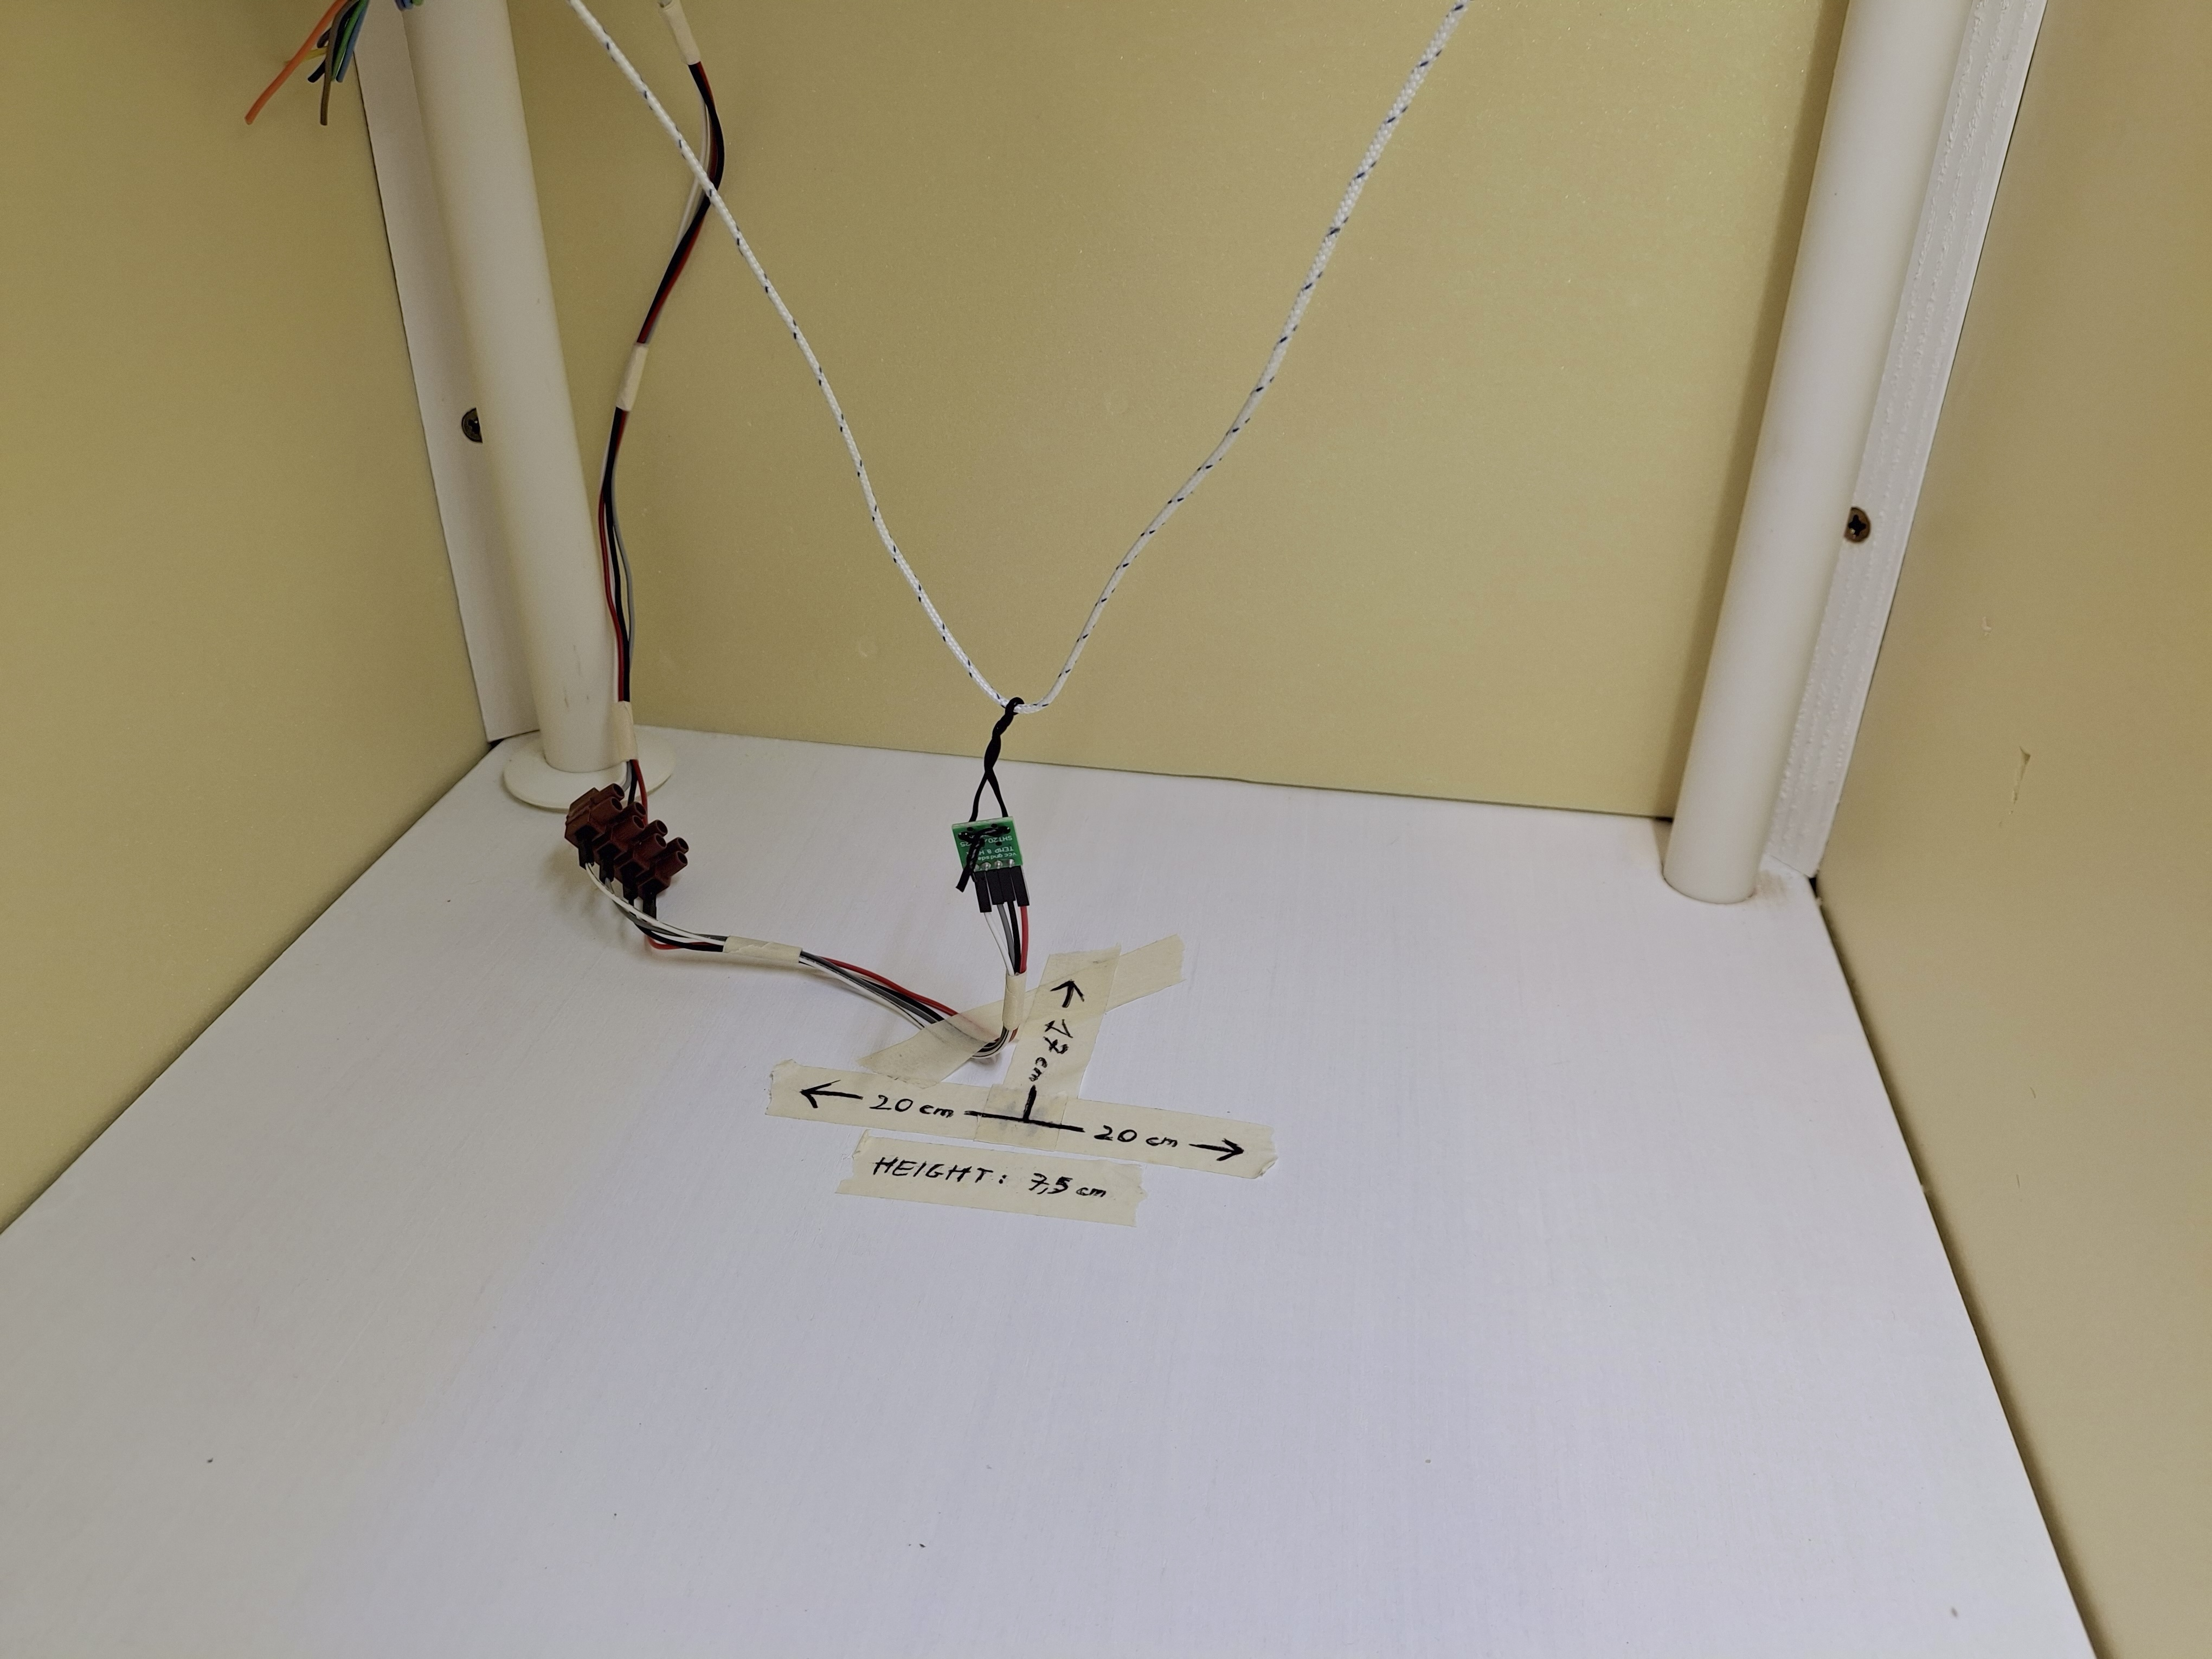
\includegraphics[width=0.9\textwidth, trim={5cm 20cm 10cm 25cm}, clip]{immagini/1_sht20.jpg}
	\caption[Foto del sensore SHT20]{Sensore di temperatura e umidità SHT20 posizionato all'interno della camera interna del
	prototipo di incubatrice neonatale.}
	\label{fig:sht20}
\end{figure}


\subsection{Scheda Arduino Mega 2560}
Per gestire i vari componenti elettronici del prototipo di incubatrice neonatale, è stata utilizzata una scheda Arduino Mega 2560
con microcontrollore ATmega2560. Essa è stata scelta per la sua semplicità d'uso, la disponibilità di numerosi pin di input/output
e l'elevato spazio di memoria disponibile per il firmware. La scheda è posizionata all'interno del cassetto inferiore del prototipo
di incubatrice neonatale, insieme a tutti i cablaggi provenienti dai vari componenti elettronici. La scheda è alimentata via USB
da un computer esterno su cui è possibile visualizzare i dati provenienti dal microcontrollore.

\begin{figure}[htbp]
	\centering
	%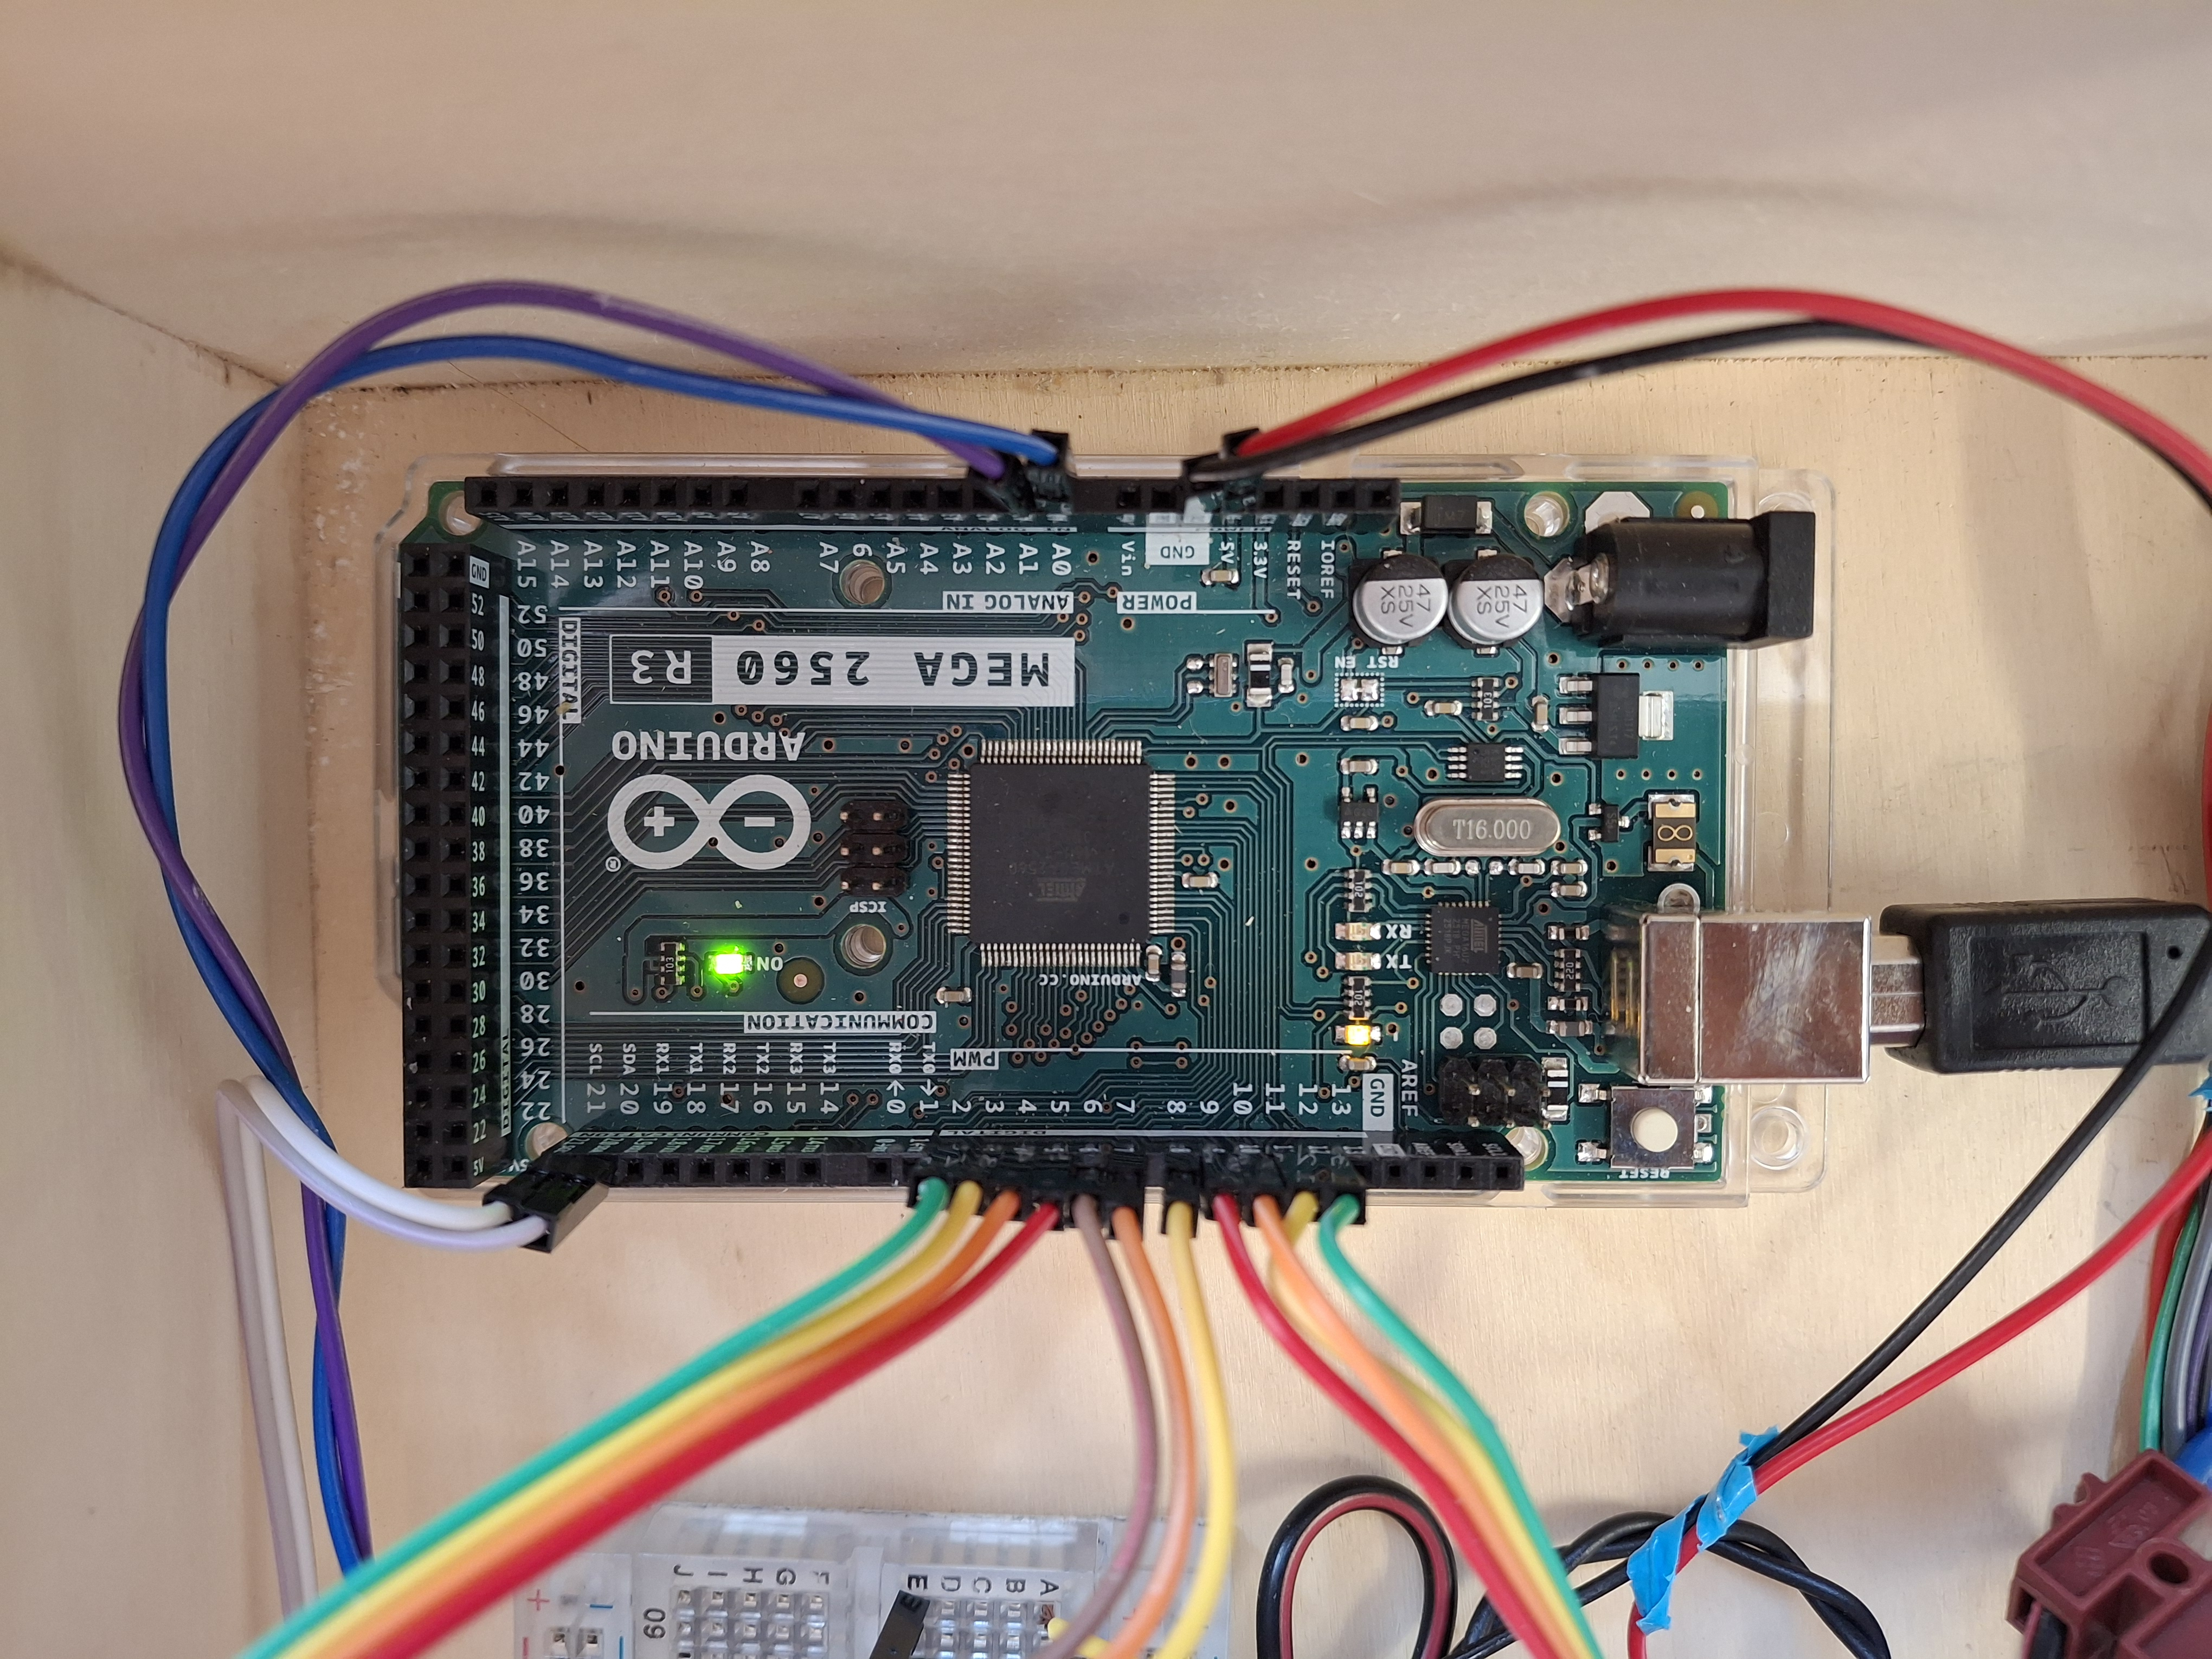
\includegraphics[width=0.9\textwidth]{immagini/1_arduino_mega.jpg}
	\caption[Foto della scheda Arduino Mega 2560]{Scheda Arduino Mega 2560 posizionata all'interno del cassetto inferiore del
	prototipo di incubatrice neonatale.}
	\label{fig:arduino_mega}
\end{figure}


\section{Collegamento delle periferiche al microcontrollore}
\subsection{Connessioni dei relè ai diversi attuatori}
Di seguito è riportato lo schema elettrico con le connessioni tra i relè e i vari attuatori presenti nel prototipo di incubatrice
neonatale realizzato con il software Fritzing. Sono indicati anche i cavi di collegamento tra i relè e la scheda Arduino, insieme
al convertitore step down per alimentare le bobine dei relè a 5 V.

Si evidenzia come l'umidificatore disponga di un suo sistema di alimentazione separato a 24 V, evidenziato dalla presenza del
tratteggio sui cavi rosso e nero. Inoltre si nota che la massa dello step down e quella dei relè non sono immediatamente collegate
tra di loro perché per distribuire la massa si utilizza la topologia a stella. Questo significa che tutti i componenti elettronici
sono collegati a un unico punto di massa (mostrato nello schema dell'Arduino), eliminando i problemi di ground lifting e riducendo
al minimo le interferenze dovute a sbalzi di corrente in corrispondenza delle commutazioni dei relè.

\begin{figure}[htbp]
	\centering
	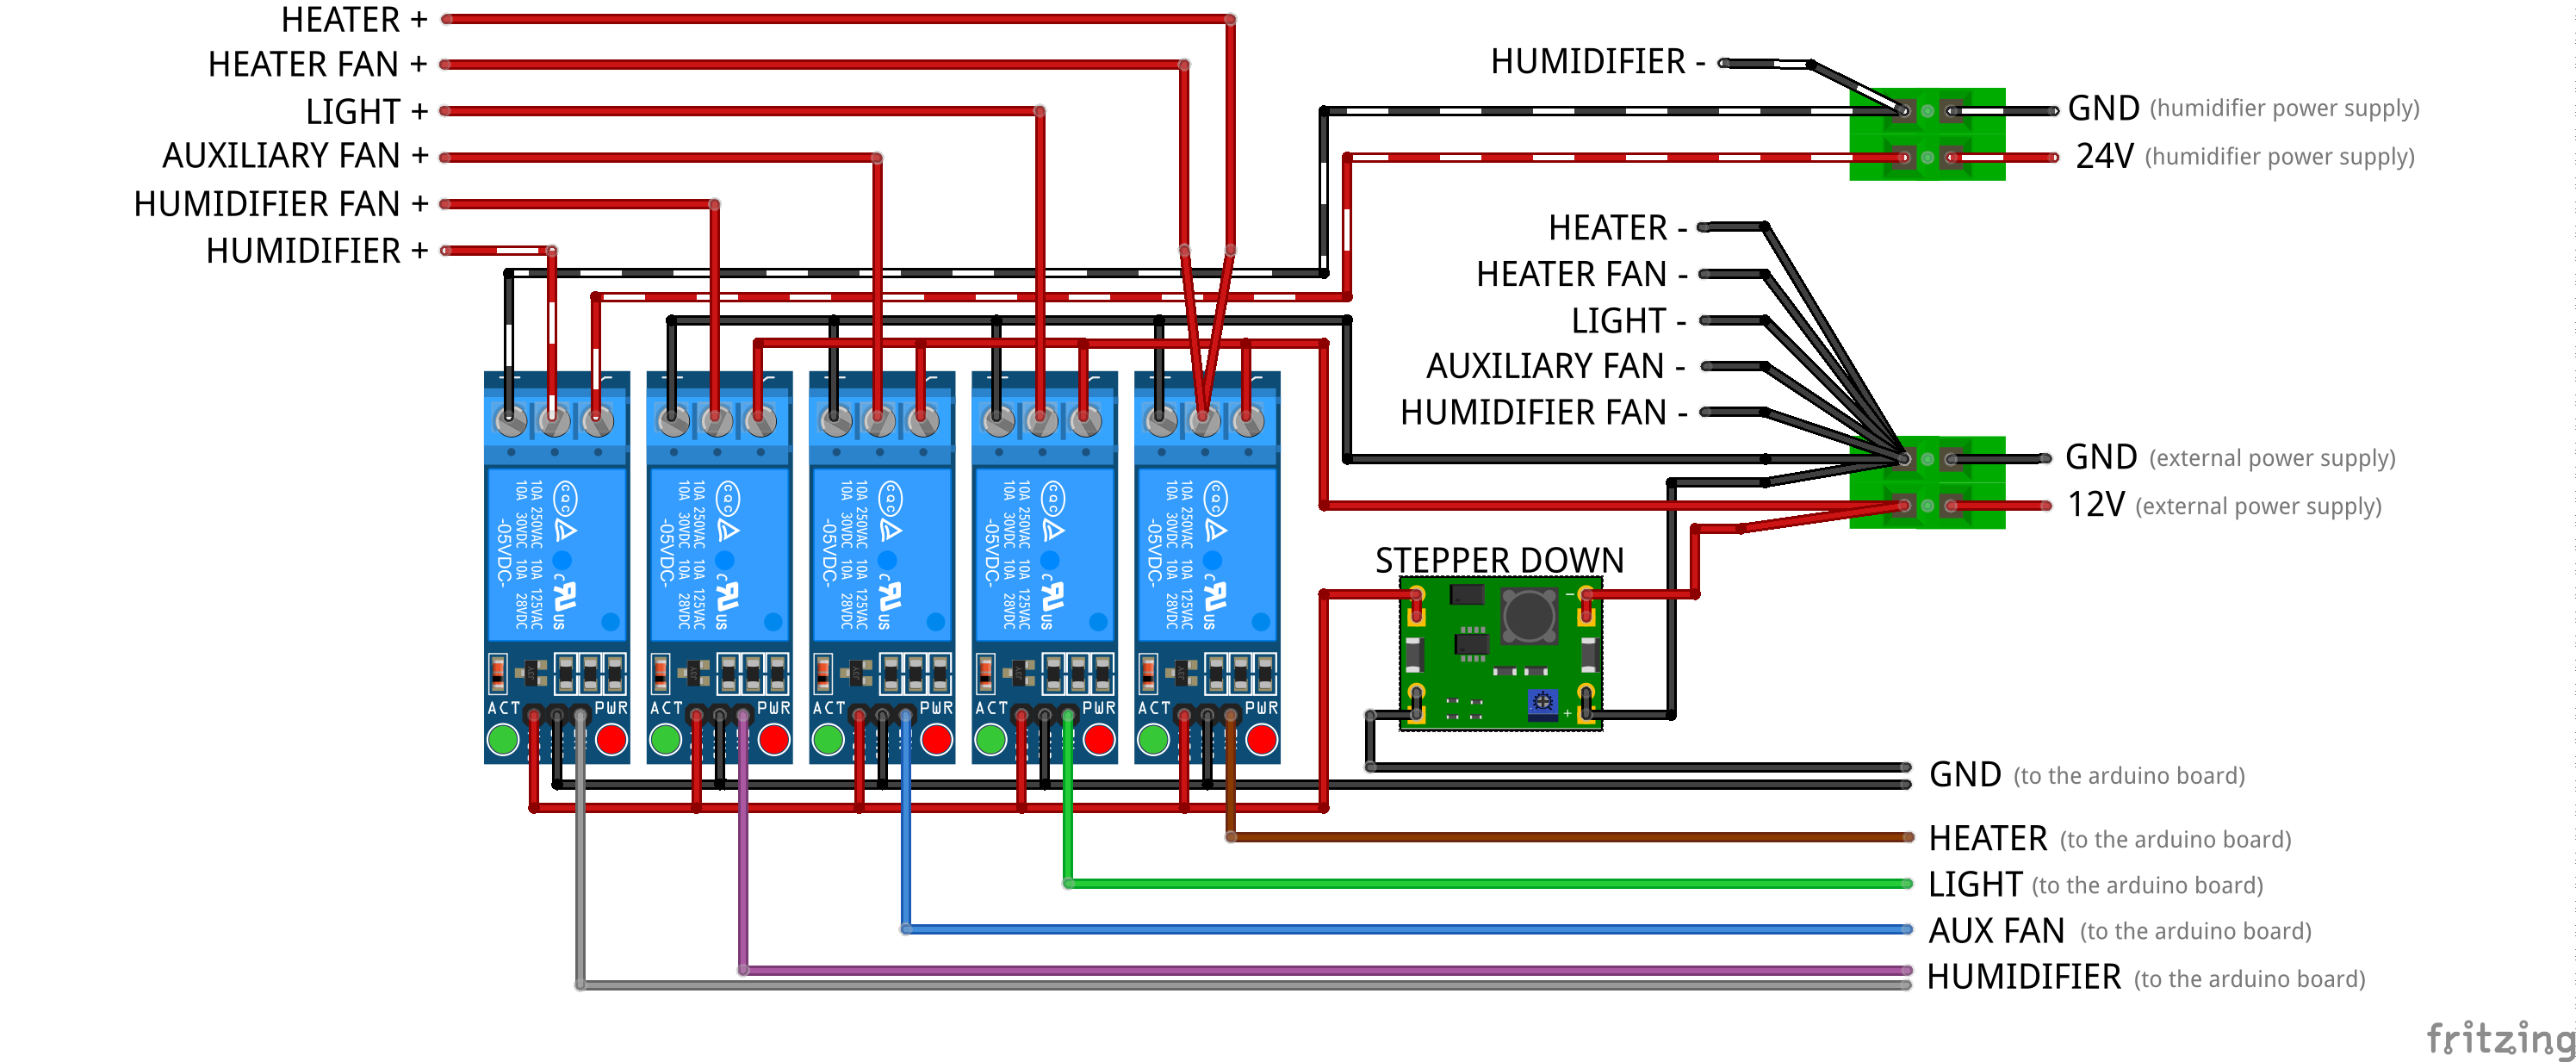
\includegraphics[width=0.9\textwidth]{immagini/1_circuito_1.png}
	\caption[Schema circuitale dei relè e degli attuatori]{Schema elettrico con le connessioni dei relè e degli attuatori
	presenti nel prototipo di incubatrice neonatale.}
	\label{fig:circuito_1}
\end{figure}

%\begin{figure}[htbp]
%	\centering
%	\includegraphics[width=0.9\textwidth]{immagini/1_foto_circuito_1.png}
%	\caption[Foto delle connessioni tra relè e attuatori]{Foto delle connessioni tra i relè e gli attuatori presenti nel
%	prototipo di incubatrice neonatale.}
%	\label{fig:foto_circuito_1}
%\end{figure}

\subsection{Connessioni del pannello frontale e del sensore SHT20}
I componenti del pannello frontale e il sensore SHT20 sono collegati al microcontrollore tramite due cavi multipolari da 10
conduttori ciascuno. Il cablaggio è alloggiato in una canalina dedicata che unisce il cassetto inferiore al pannello frontale
e alla camera interna dell'incubatrice.

Al fine di garantire affidabilità e agevolare le future operazioni di manutenzione, le connessioni verso il pannello frontale
sono state modularizzate utilizzando dei connettori JST disponibili in laboratorio. In particolare sono stati scelti tre connettori
a 4 pin per i segnali di controllo e un connettore a 2 pin per l'alimentazione. Le connessioni interne tra i componenti del pannello
frontale, la catena di alimentazione e i rispettivi connettori sono state saldate con stagno per garantire un collegamento stabile
e duraturo nel tempo.

Il sensore SHT20, per mantenere una certa flessibilità nella sua posizione all'interno della camera interna, è stato collegato
ai cavi della canalina tramite una serie di 4 morsetti mammuth. In questo modo è possibile scollegare il sensore, allungare o
accorciare i cavi per poter posizionare agevolmente il sensore in diverse posizioni.

Per maggiore leggibilità, è stato scelto di tratteggiare i conduttori del cavo multipolare che collega il sensore SHT20 e il
led di refill al microcontrollore. Si nota che non tutti i conduttori di questo cavo sono stati utilizzati.

\begin{figure}[htbp]
    \centering
    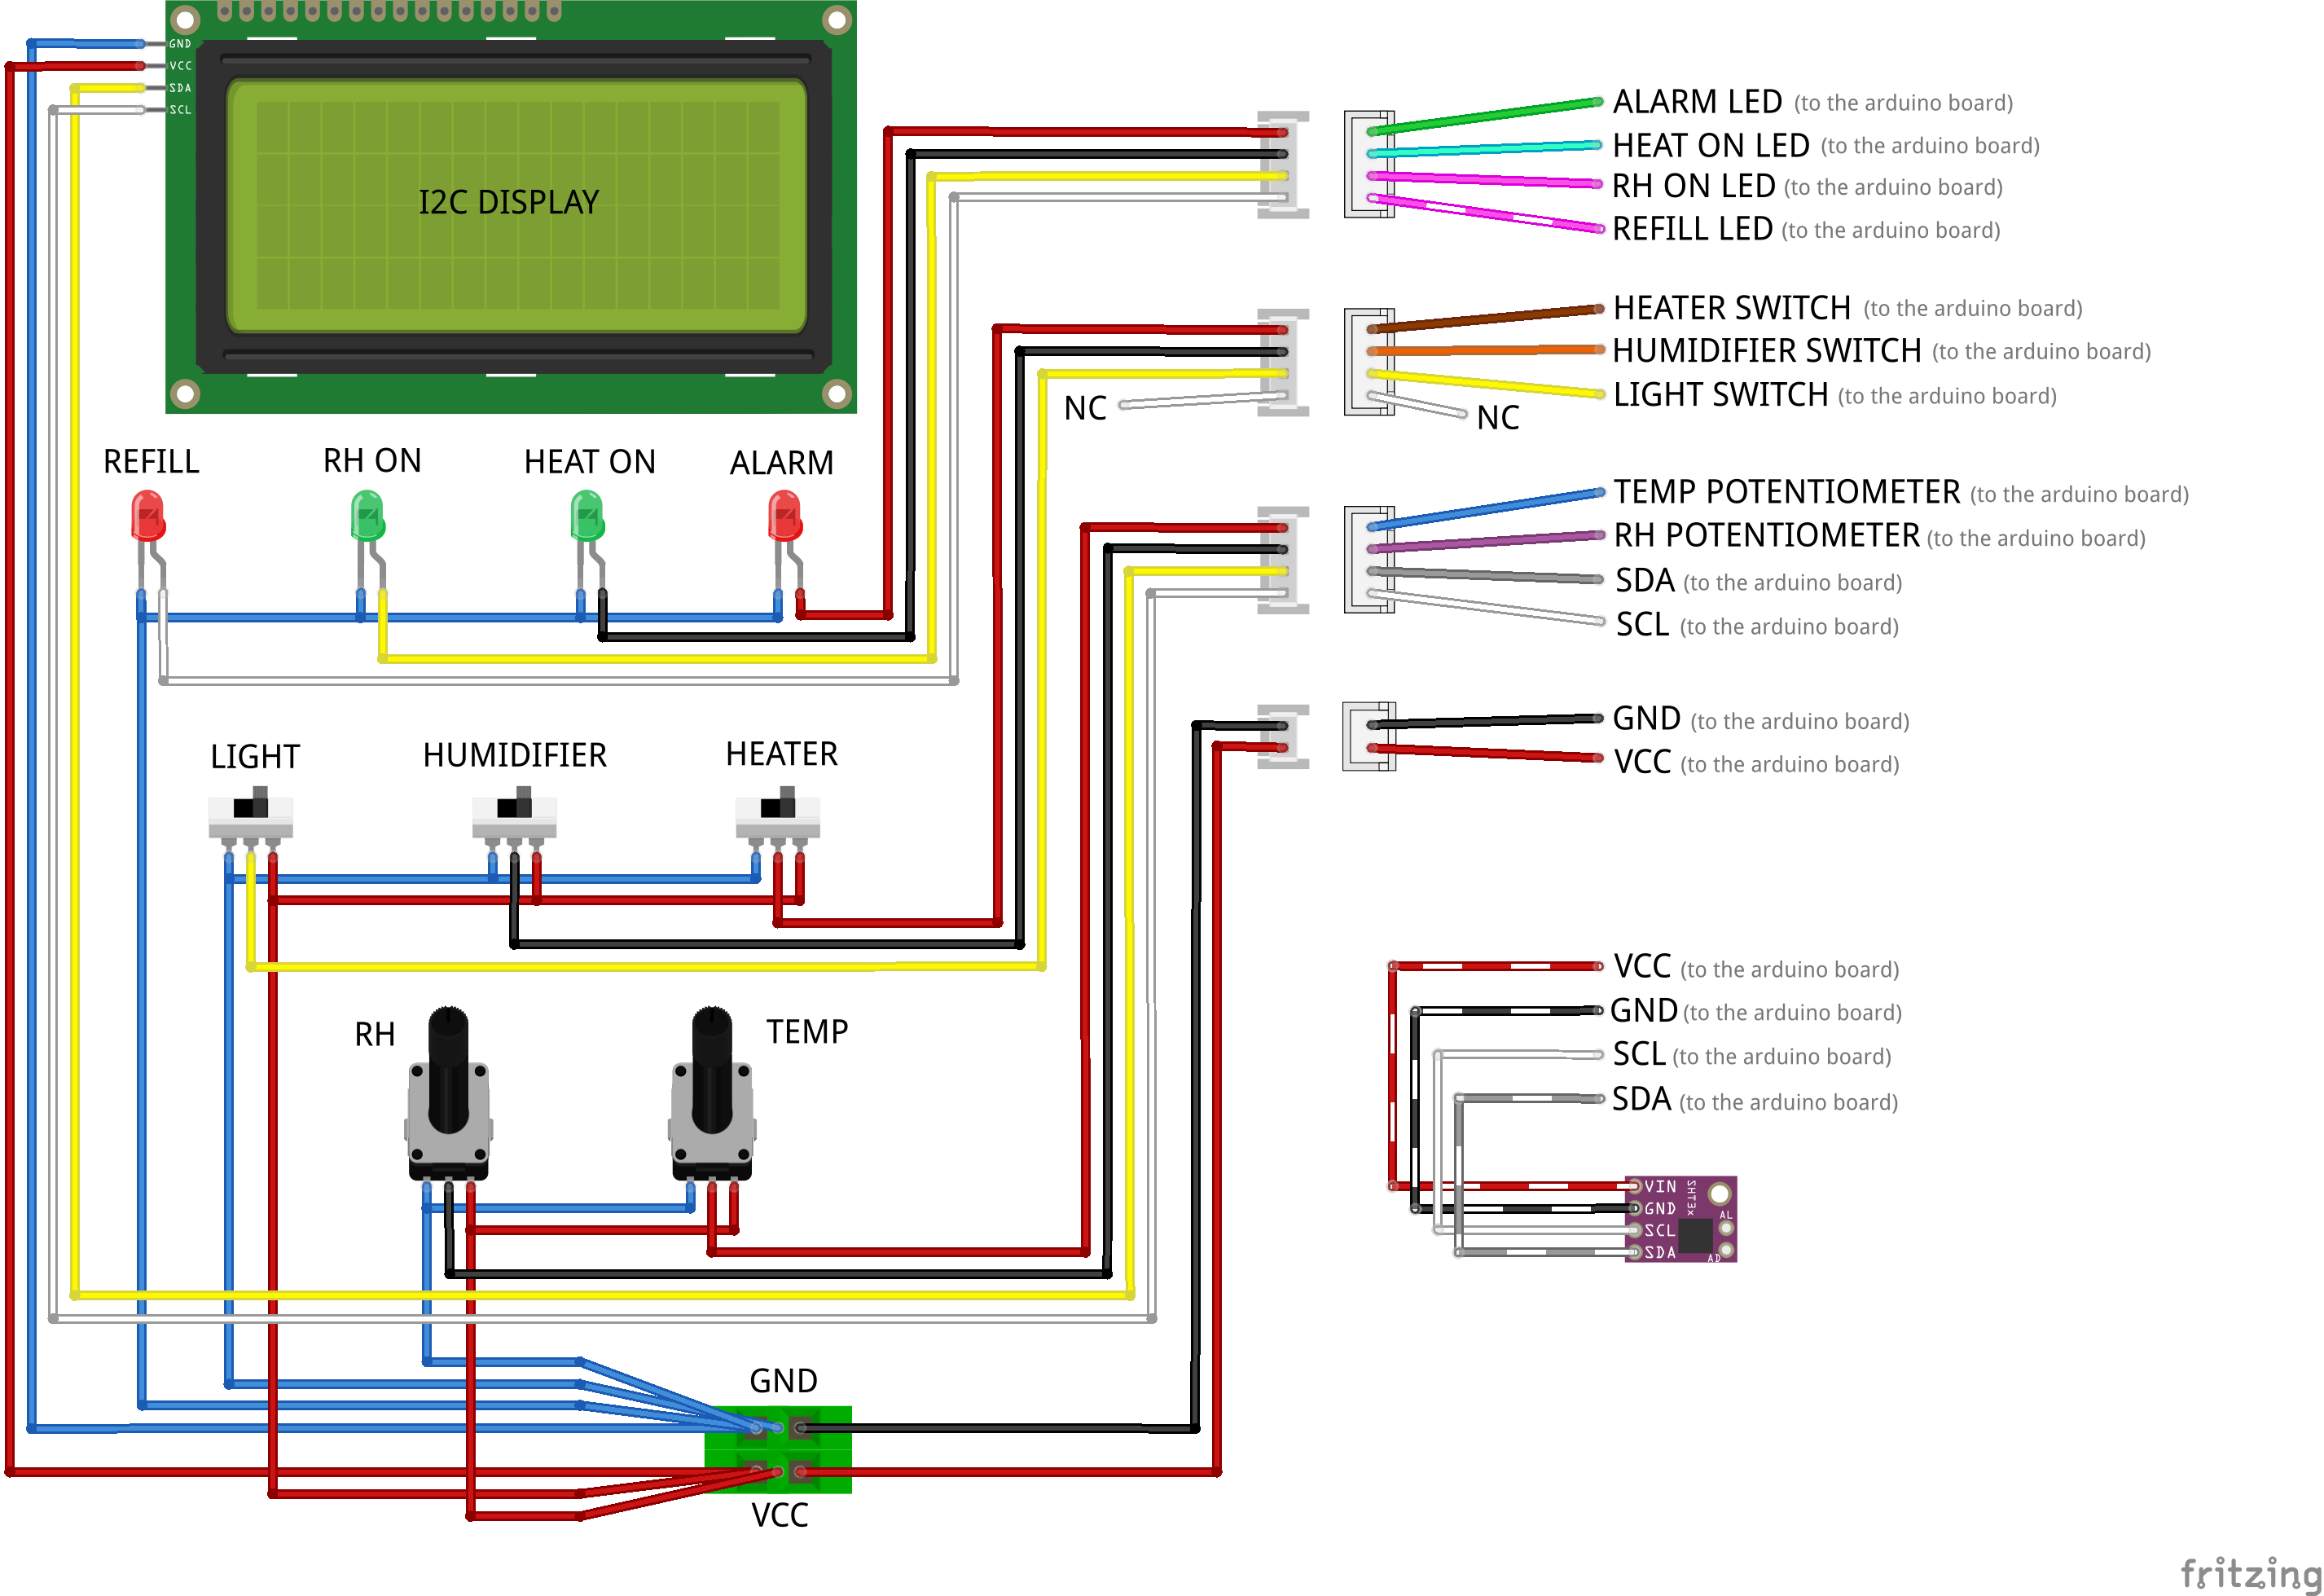
\includegraphics[width=0.9\textwidth]{immagini/1_circuito_2.png}
    \caption[Schema circuitale del pannello frontale e del sensore SHT20]{Schema elettrico con le connessioni del sensore di
	temperatura e umidità SHT20 e dei vari componenti presenti nel pannello frontale del prototipo di incubatrice neonatale.}
    \label{fig:circuito_2}
\end{figure}

%\begin{figure}[htbp]
%    \centering
%    \includegraphics[width=0.9\textwidth]{immagini/1_foto_circuito_2.png}
%    \caption[Foto delle connessioni nel pannello frontale]{Foto delle connessioni tra i vari componenti presenti nel pannello
%	frontale del prototipo di incubatrice neonatale.}
%    \label{fig:foto_circuito_2}
%\end{figure}

\subsection{Connessioni dei vari componenti al microcontrollore}
Nel seguente schema elettrico sono riportate tutte le connessioni tra i cavi multipolari provenienti dai vari componenti
del prototipo e i cavi di controllo dei relè con i pin del microcontrollore. Si nota la presenza del nodo principale di massa
a cui convergono tutti i cavi di massa dei vari componenti.

Per limitare la corrente nei led di stato del pannello frontale, sono state inserite delle resistenze di bias. I relativi valori
sono stati calcolati in modo da garantire una corrente di circa 10 mA e sono poi state aggiustate in maniera empirica per ottenere
una luminosità dei led adeguata. Di seguito sono riportati i valori e le misurazioni effettive della corrente nei led di stato.
Si nota come le resistenze dei led di colore rosso siano più alte rispetto a quelle dei led di colore verde, in quanto, a parità
di corrente, i led rossi risultano più luminosi rispetto a quelli verdi.

\begin{table}[htbp]
	\centering
	\begin{tabular}{c | c | c}
		\textbf{Led} & \textbf{Resistenza} & \textbf{Corrente} \\
		\toprule
		Allarme (rosso) & 470 $\Omega$ & 6.10 mA \\
		\midrule
		Riscaldatore (verde) & 220 $\Omega$ & 12.2 mA \\
		\midrule
		Umidificatore (verde) & 220 $\Omega$ & 12.2 mA \\
		\midrule
		Refill (rosso) & 470 $\Omega$ & 6.11 mA
	\end{tabular}
	\caption{Valori e misurazioni della corrente nei led di stato}
	\label{tab:led_current}
\end{table}

\begin{figure}[htbp]
    \centering
    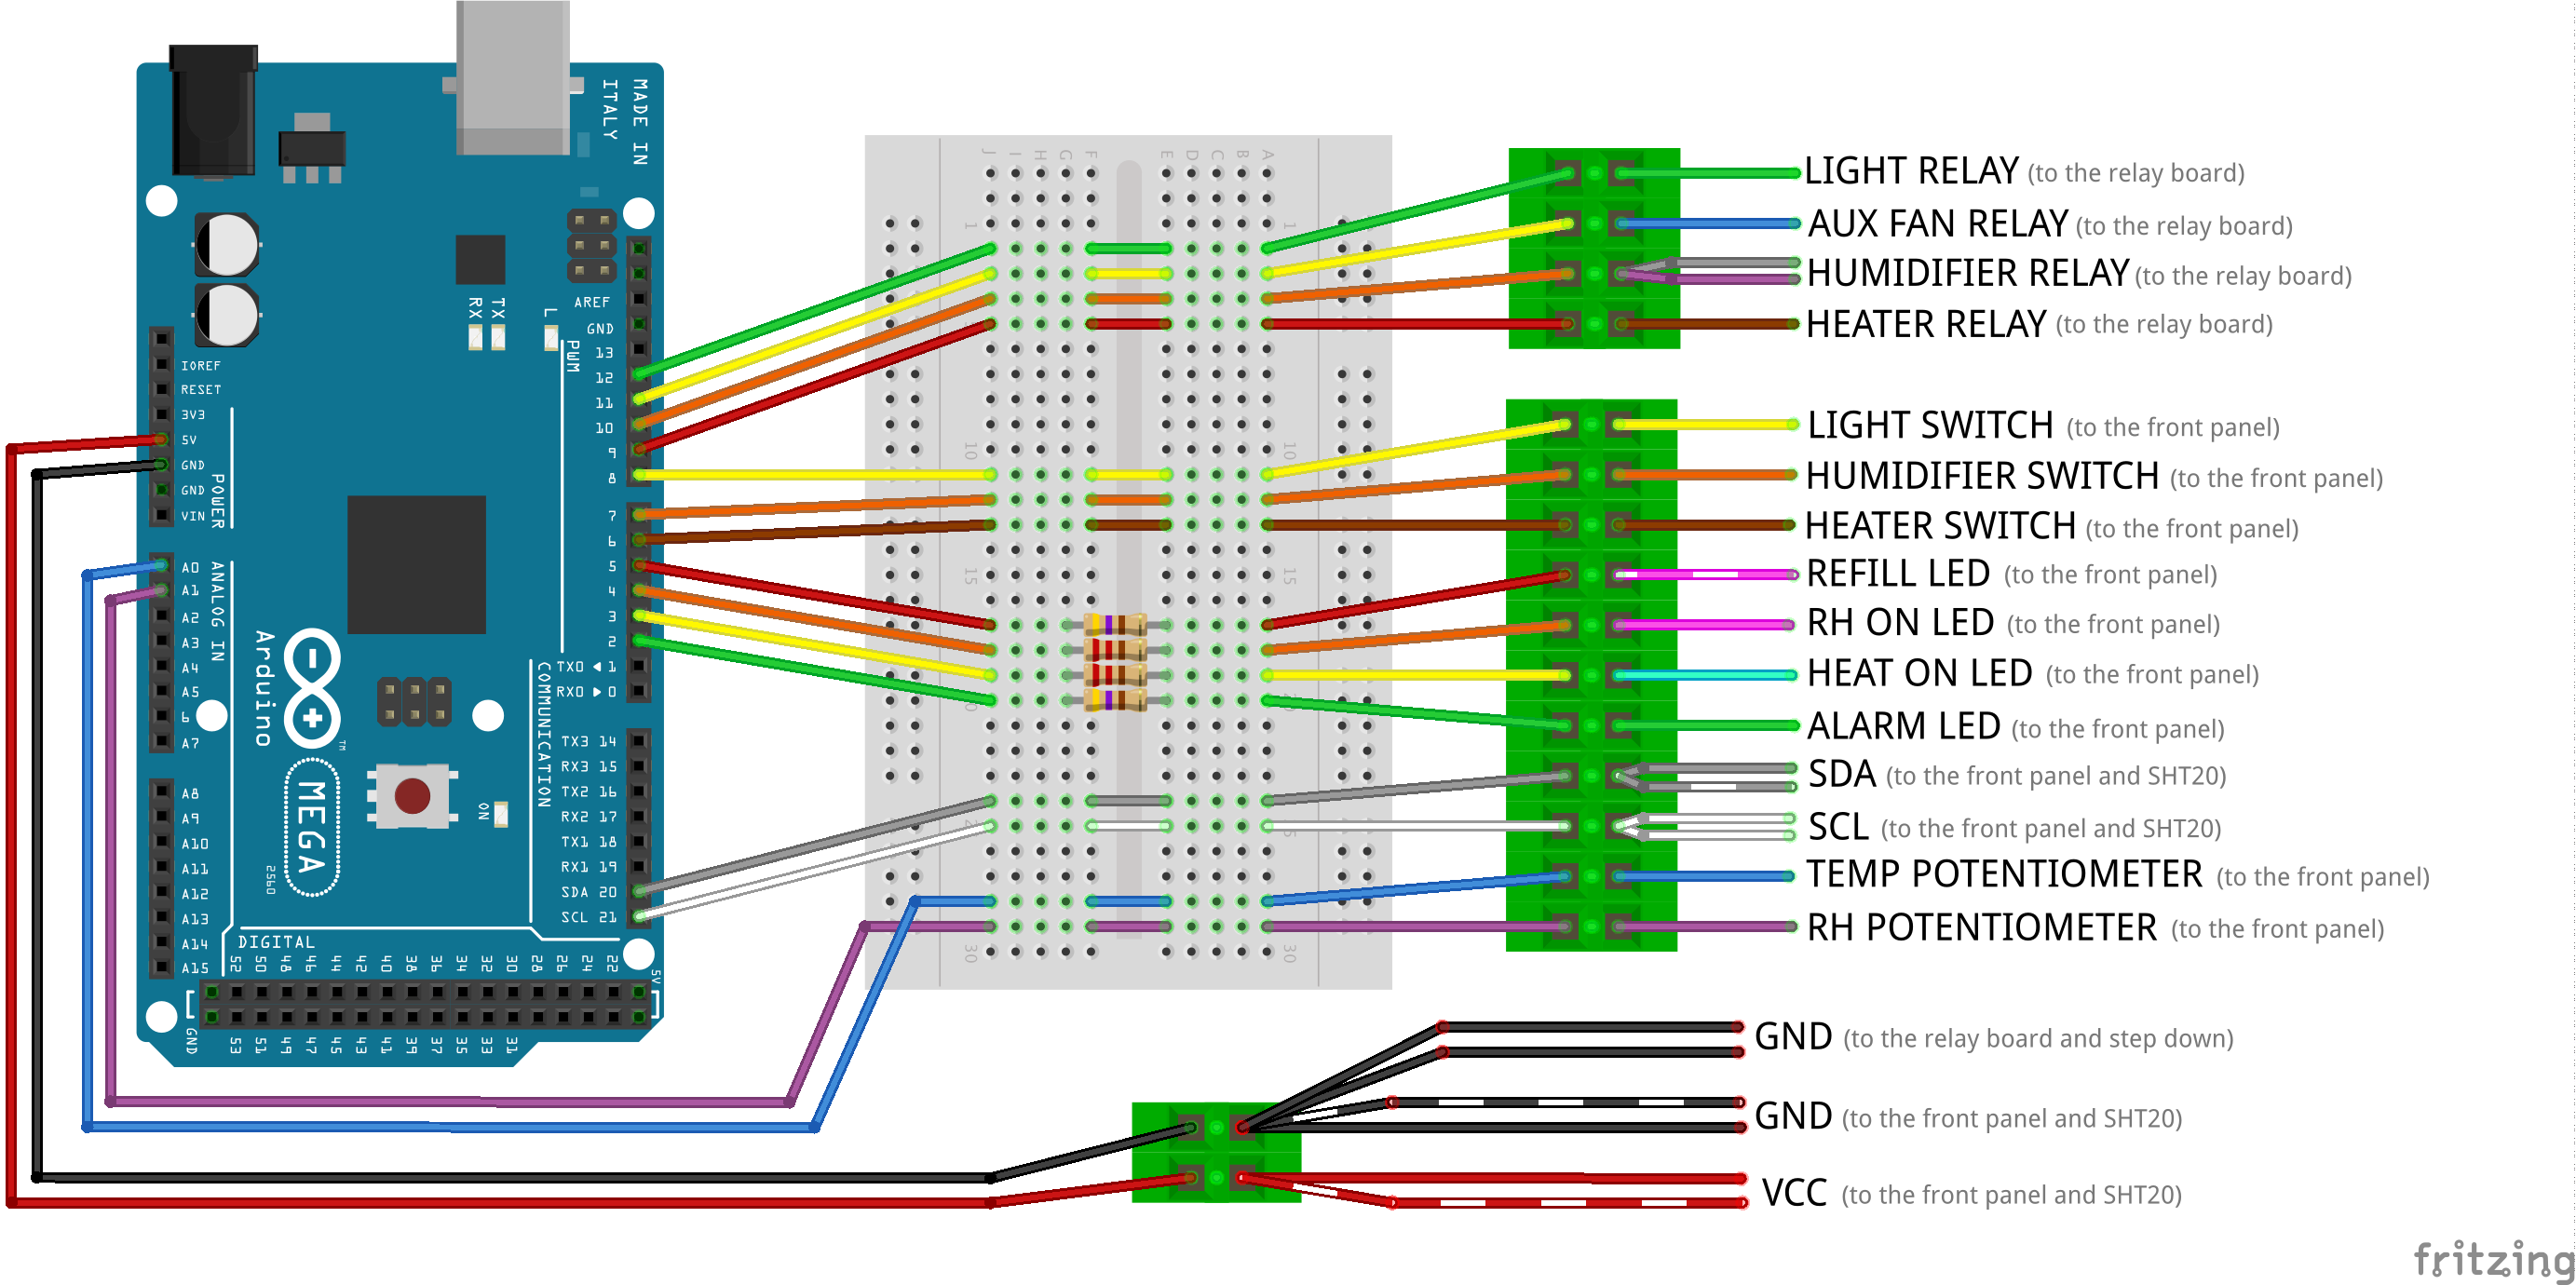
\includegraphics[width=0.9\textwidth]{immagini/1_circuito_3.png}
    \caption[Schema circuitale del microcontrollore]{Schema elettrico con le connessioni dei cavi provenienti dai vari componenti
	al microcontrollore Arduino Mega 2560.}
    \label{fig:circuito_3}
\end{figure}

%\begin{figure}[htbp]
%    \centering
%    %\includegraphics[width=0.9\textwidth]{immagini/1_foto_circuito_3.png}
%    \caption[Foto delle connessioni del microcontrollore]{Foto delle connessioni dei cavi provenienti dai vari componenti
%	al microcontrollore Arduino Mega 2560.}
%    \label{fig:foto_circuito_3}
%\end{figure}

\begin{figure}[htbp]
    \centering
    %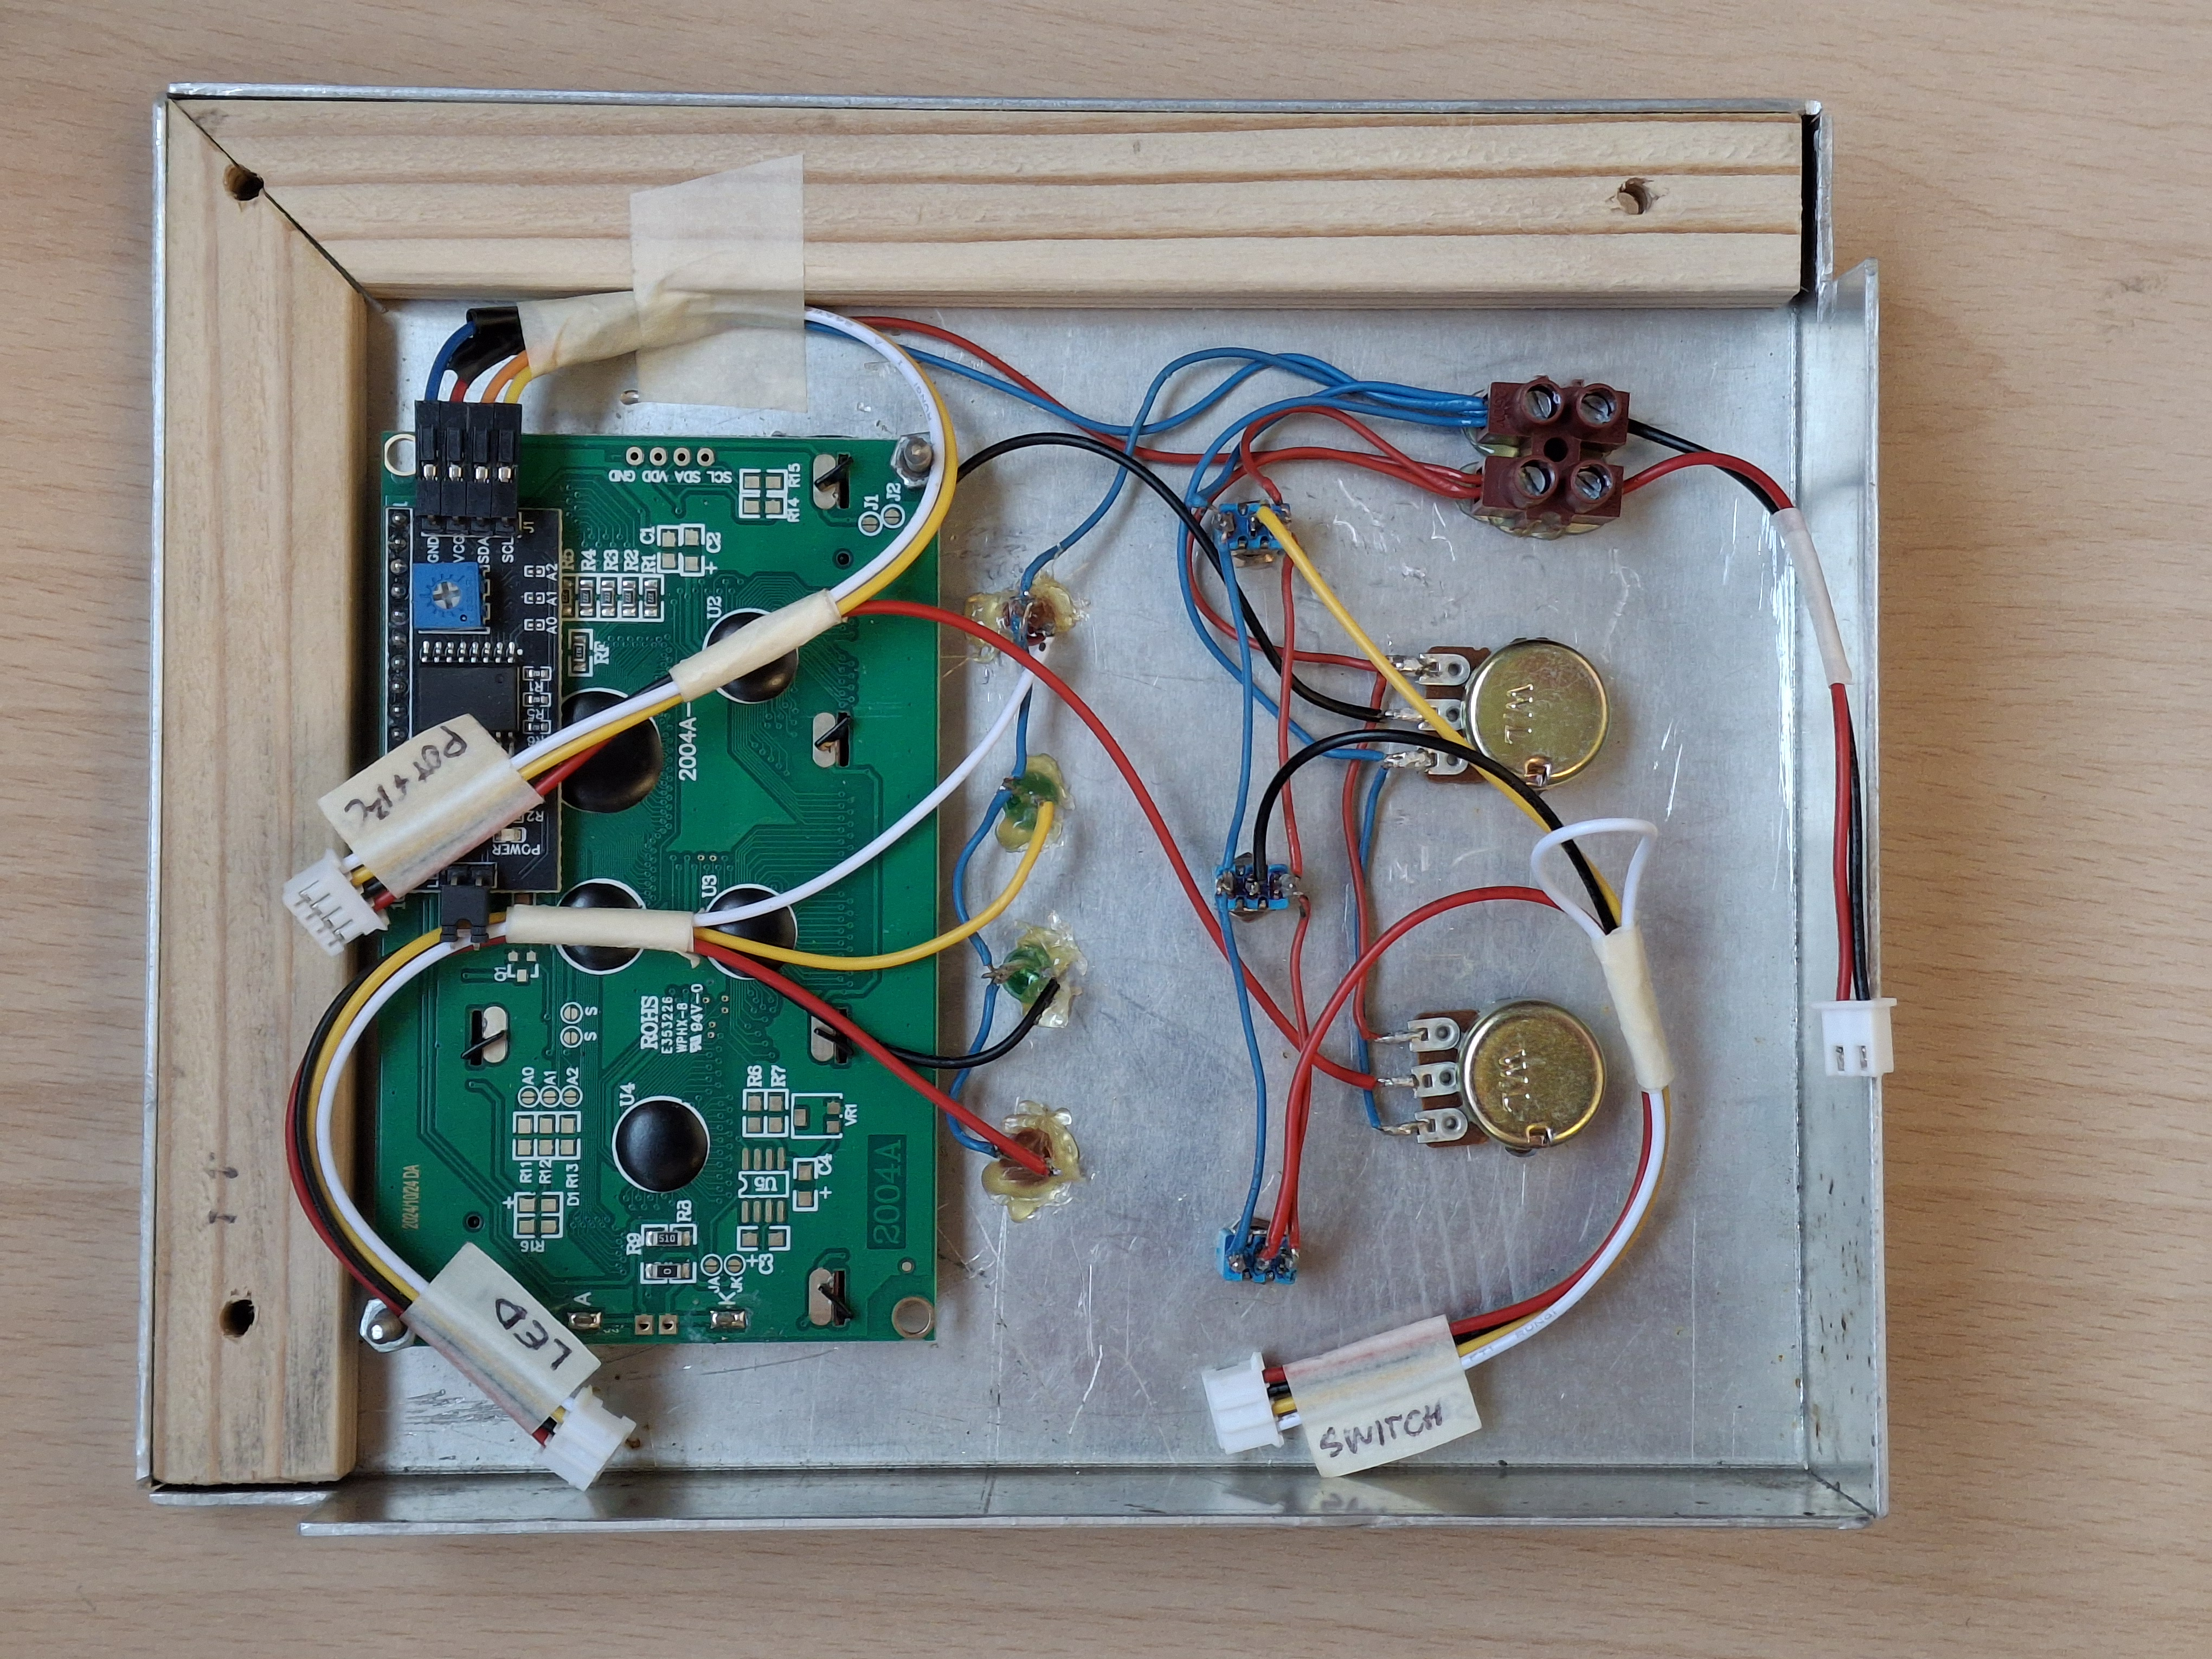
\includegraphics[width=0.9\textwidth]{immagini/1_pannello_frontale_2.png}
    \caption[Foto delle connessioni nel pannello frontale]{Foto delle connessioni tra i vari componenti presenti nel pannello
	frontale del prototipo di incubatrice neonatale.}
    \label{fig:foto_circuito_2}
\end{figure}

\begin{figure}[htbp]
    \centering
    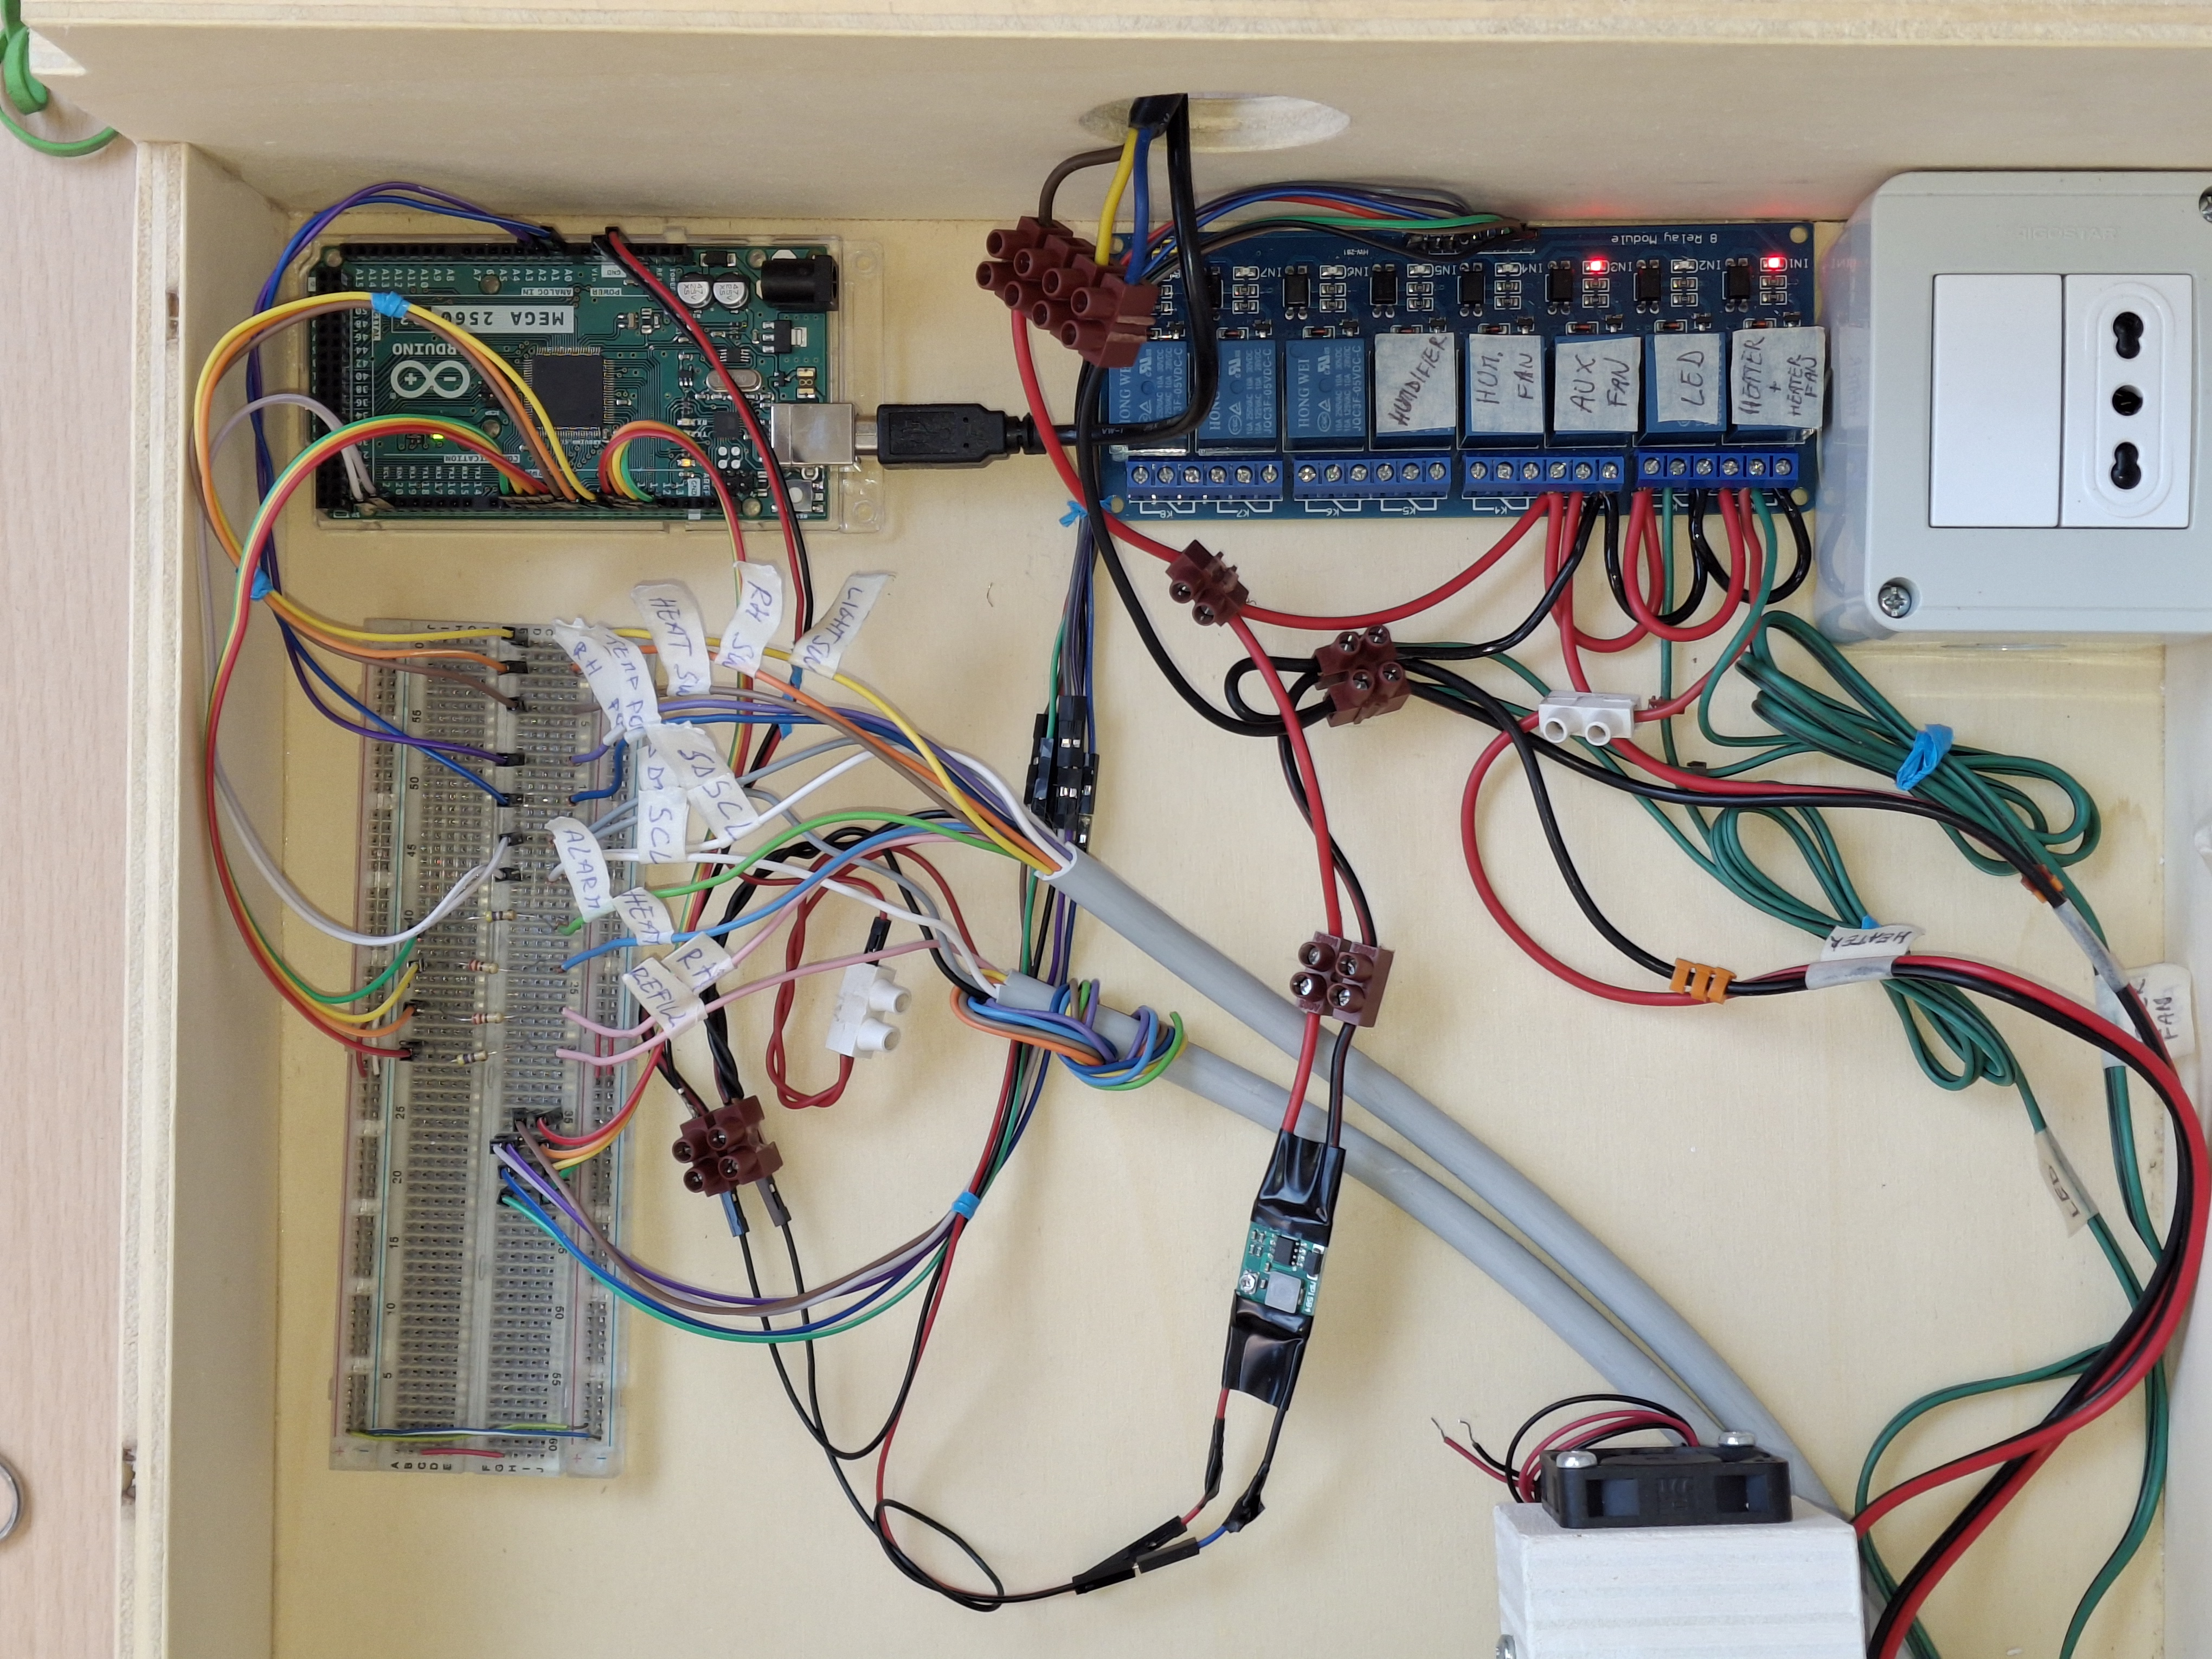
\includegraphics[width=0.9\textwidth]{immagini/1_cassetto.jpg}
    \caption[Foto delle connessioni del cassetto]{Foto delle connessioni presenti nel cassetto inferiore del prototipo di
	incubatrice neonatale in cui si possono notare la scheda Arduino Mega 2560, il modulo relè, lo step down, i cavi provenienti
	dal pannello frontale e dal sensore, la breadboard dove convergono tutti i cavi e il morsetto marrone per la distribuzione
	della massa.}
    \label{fig:foto_circuito_3}
\end{figure}
